\documentclass[11pt,a4 paper,one side]{article}
\usepackage{amsmath,amssymb,graphicx,subcaption}
\usepackage{ctex}  
\usepackage[colorlinks=true,linkcolor=red,citecolor=red,filecolor=magenta,urlcolor=cyan]{hyperref}
\usepackage{bookmark}
\usepackage{fontspec}
\setmainfont{Times New Roman}
\usepackage{xcolor}
\usepackage{geometry}
\geometry{a4paper, left=2.5cm, right=2.5cm, top=2.5cm, bottom=2.5cm}
\title{科学机器学习+HW3报告}
\author{2100012131 蒋鹏}
\date{\today}
\begin{document}
\maketitle
\tableofcontents
\section{全连接神经网络}
\subsection{问题描述}
考虑$R\rightarrow R$的线性函数$y=x$，随机生成1000个$[-1,1]$上的数据$\{x_i,y_i\}$，使用$\sigma$=ReLU作为激活函数的两层神经网络
\begin{equation}
    f(x)=W^{(2)}\sigma (W^{(1)}x+b^{(1)})+b^{(2)}
\end{equation}
进行拟合。自己尝试不同的$D$进行训练，并对$x\in[-10,10]$进行预测。线性函数$y=x$能被两层神经网络精确表示吗？如果可以，神经网络的训练能找到这样的精确表示吗？
考虑二次函数$y=x^2$和高频函数$y=\sin(10\pi x)$，重复上述练习。
\subsection{数值方法}
使用pytorch搭建神经两层神经网络，激活函数为$\sigma$=ReLU，损失函数使用均方误差MSEloss，优化器为Adam。为了简单，设定随机种子为42号。
\subsection{线性函数}
\subsubsection{参数设置}
学习率lr=0.001，epoch=2000，D=[2, 5, 10, 20, 100, 500]。
\subsubsection{数值结果}
首先用表格展示数值结果。
\begin{table}
    \centering
    \begin{tabular}{c c c c c}
        \hline
        D&内插最大误差&内插平均误差&外推最大误差&外推平均误差\\
        2&0.226&0.014&10.7&2.7\\
        5&0.137&7.1e-3&9.1&2.3\\
        10&3.5e-2&5e-3&2.9&1.2\\
        20&1.5e-2&2.7e-3&4.2&1.3\\
        100&2.8e-3&7e-4&2.0&0.96\\
        500&1.6e-3&3.9e-4&0.68&0.20\\
    \end{tabular}
    \caption{线性函数}
    \label{线性函数}
\end{table}
下面用图片展示数值结果，包括真实函数与预测函数曲线对比、预测误差曲线、训练Loss下降曲线。
\begin{figure}[htbp]
    \centering
    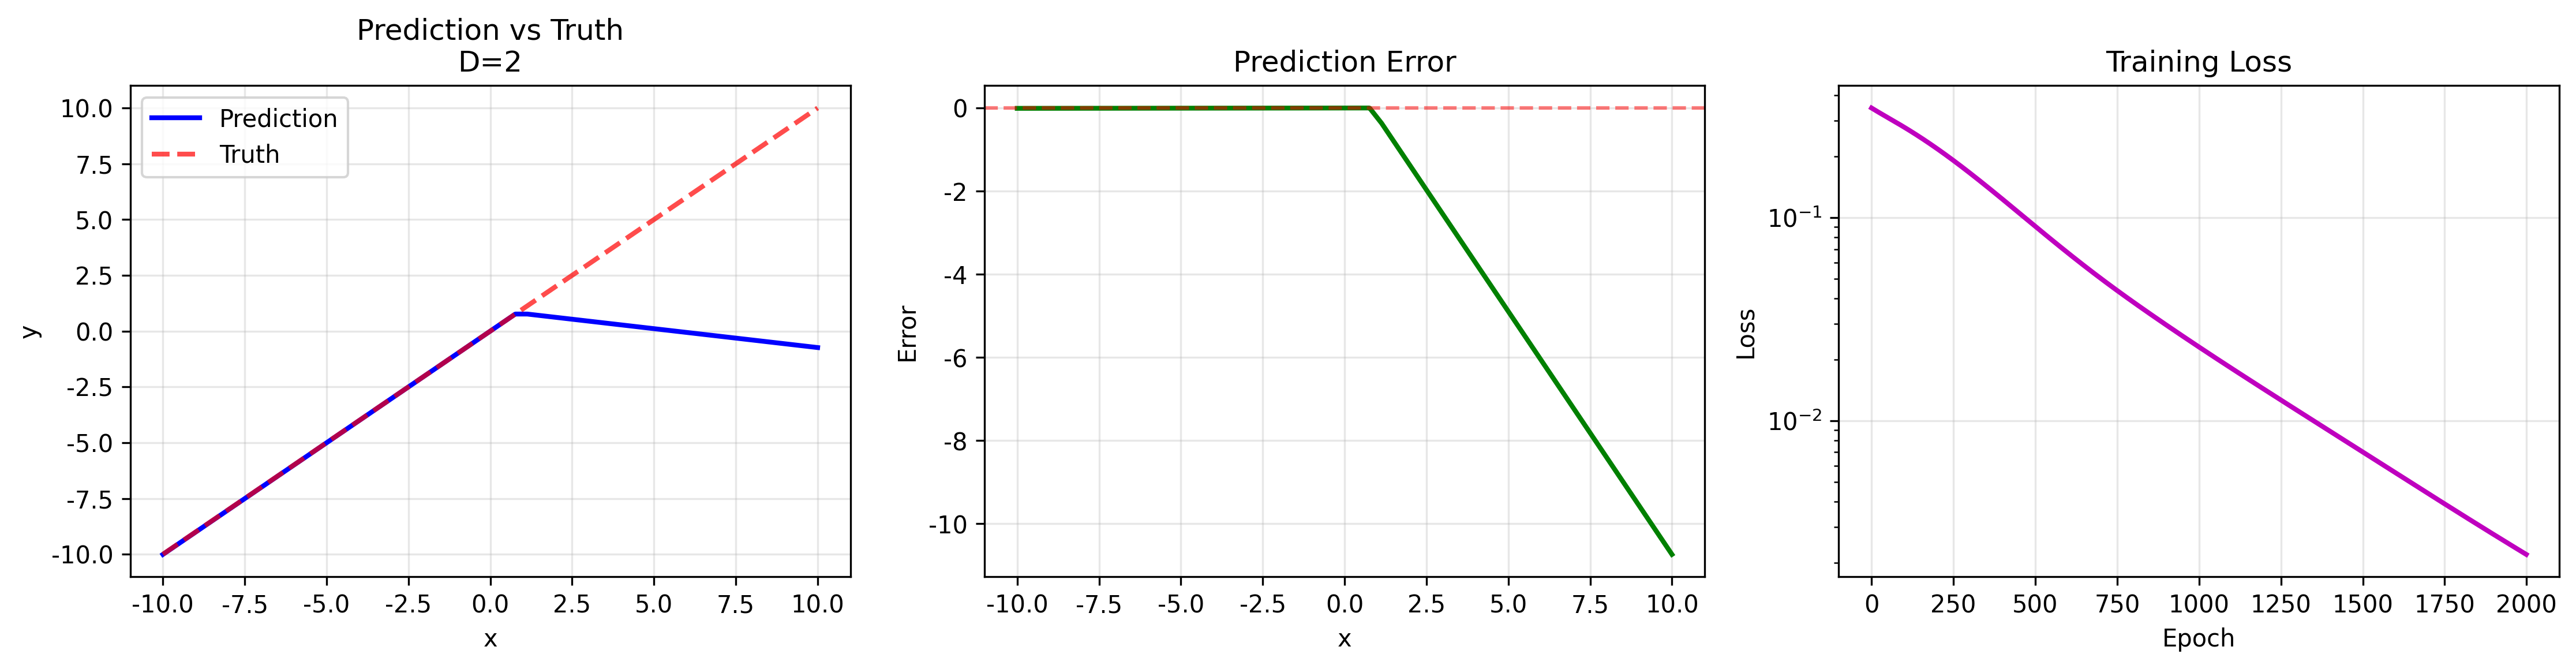
\includegraphics[width=\linewidth]{linear D2.png}
    \caption{linear D2}
    \label{linear D2}
\end{figure}
\begin{figure}[htbp]
    \centering
    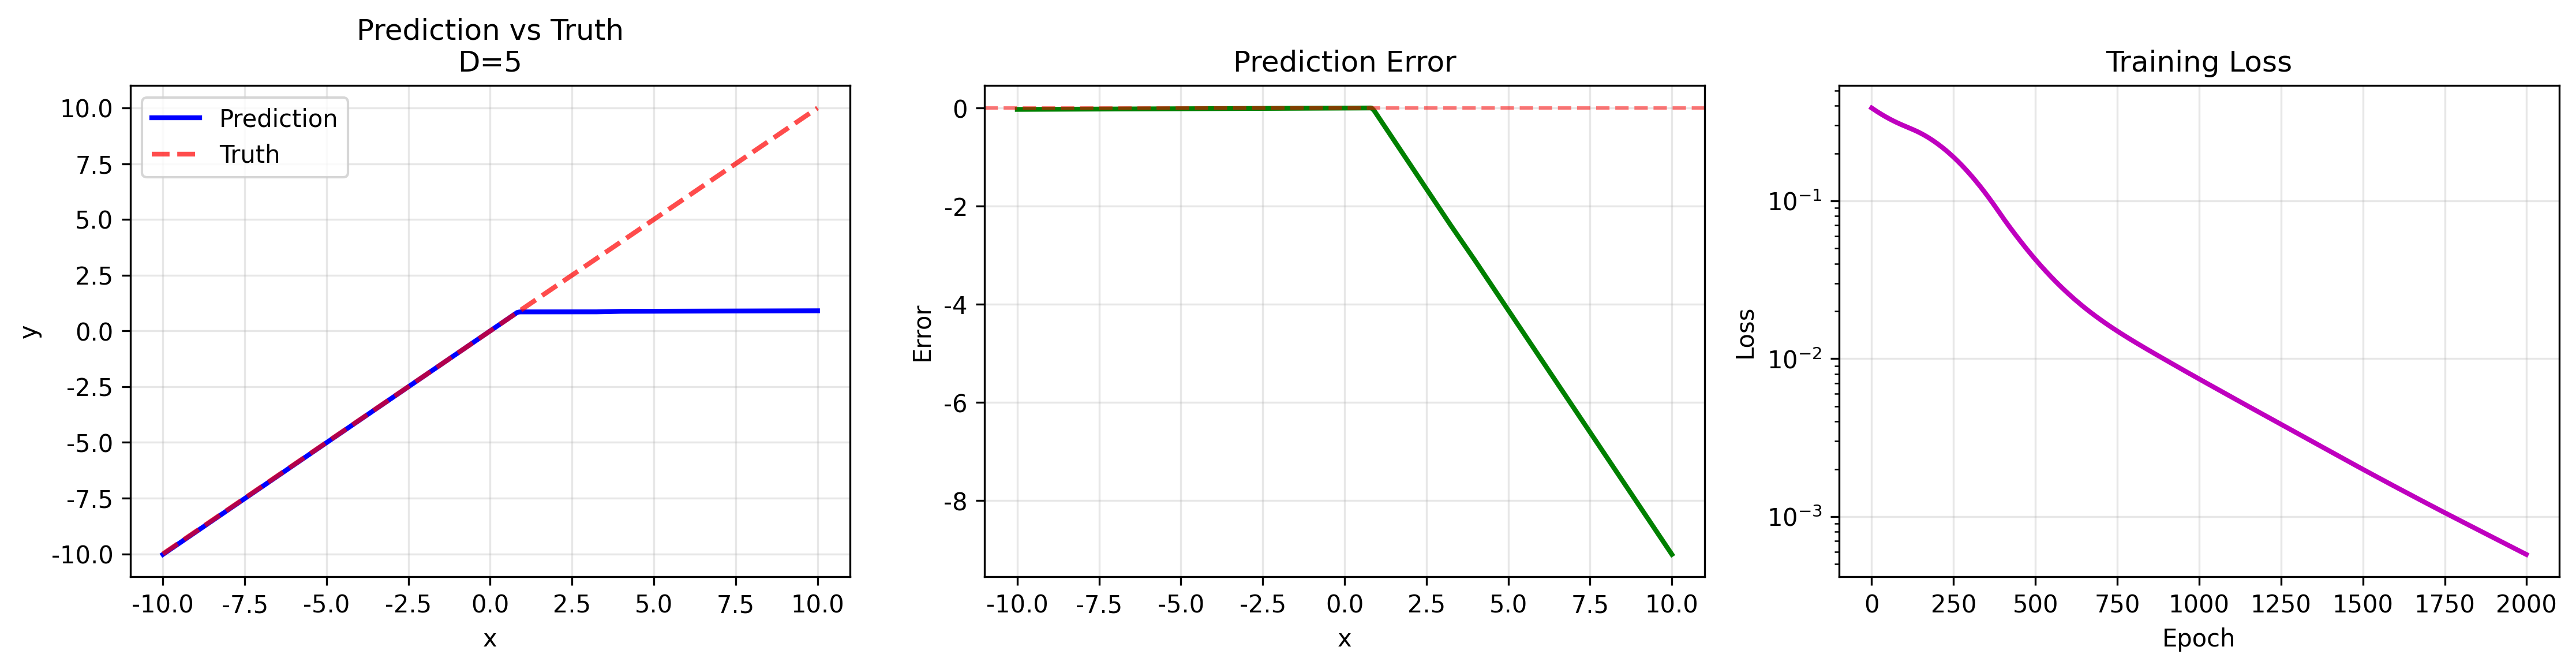
\includegraphics[width=\linewidth]{linear D5.png}
    \caption{linear D5}
    \label{linear D5}
\end{figure}
\begin{figure}[htbp]
    \centering
    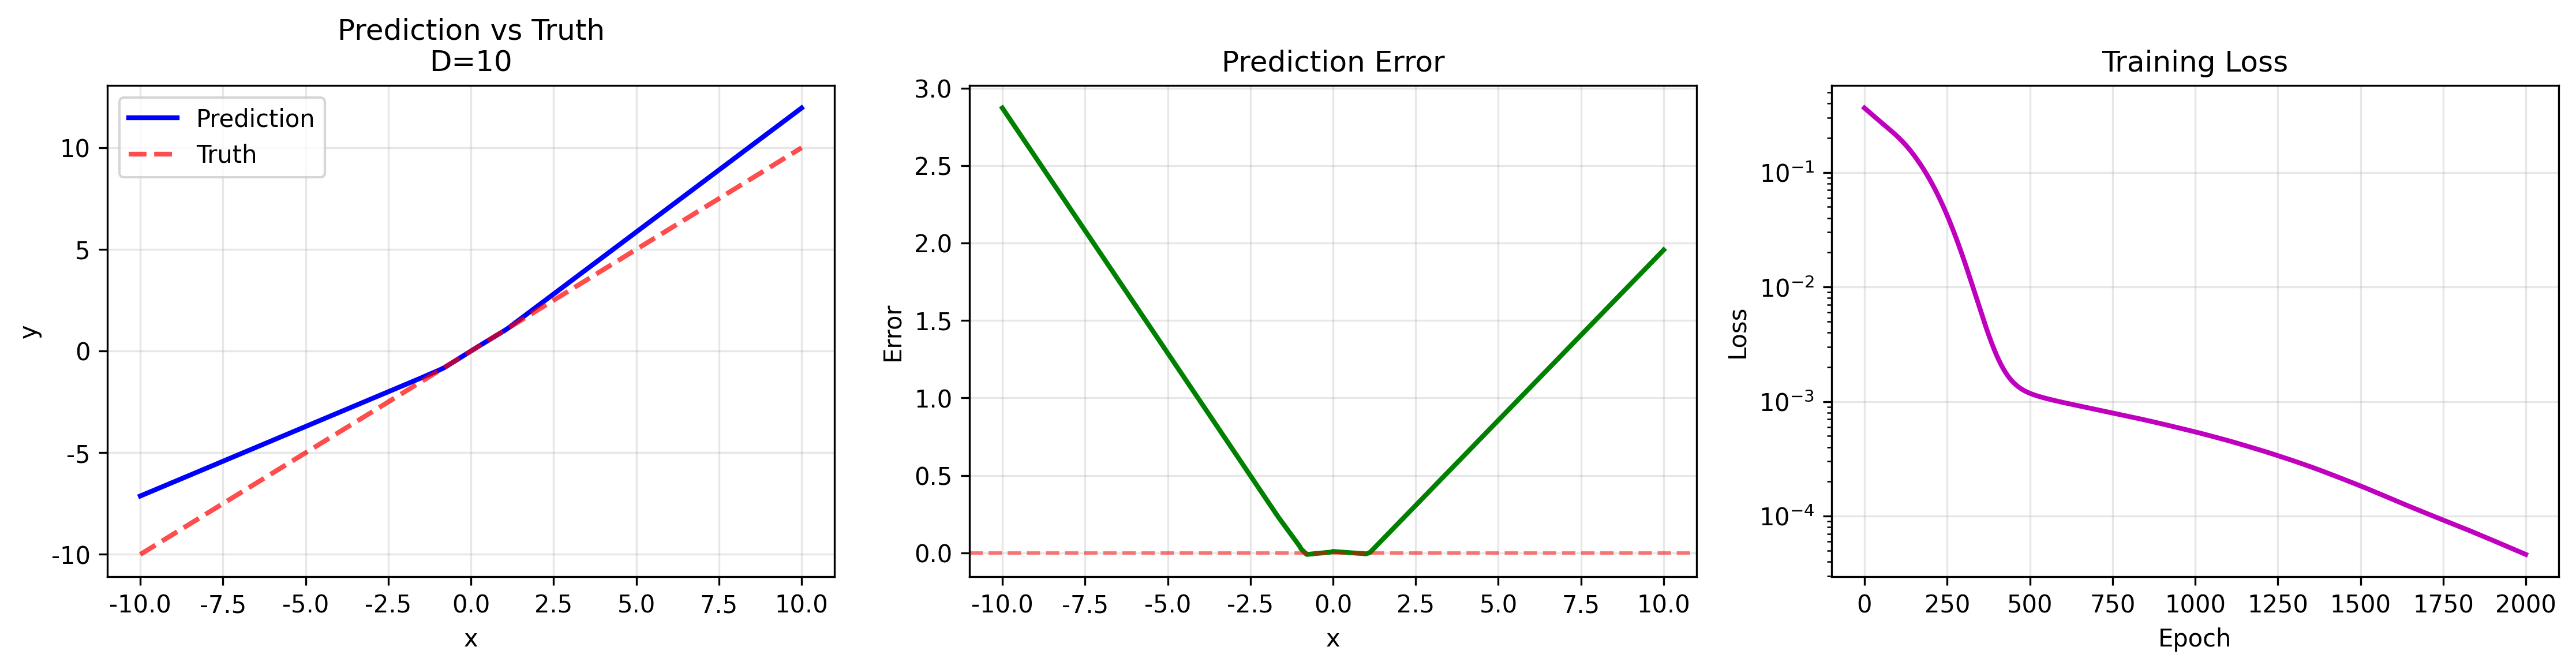
\includegraphics[width=\linewidth]{linear D10.png}
    \caption{linear D10}
    \label{linear D10}
\end{figure}
\begin{figure}[htbp]
    \centering
    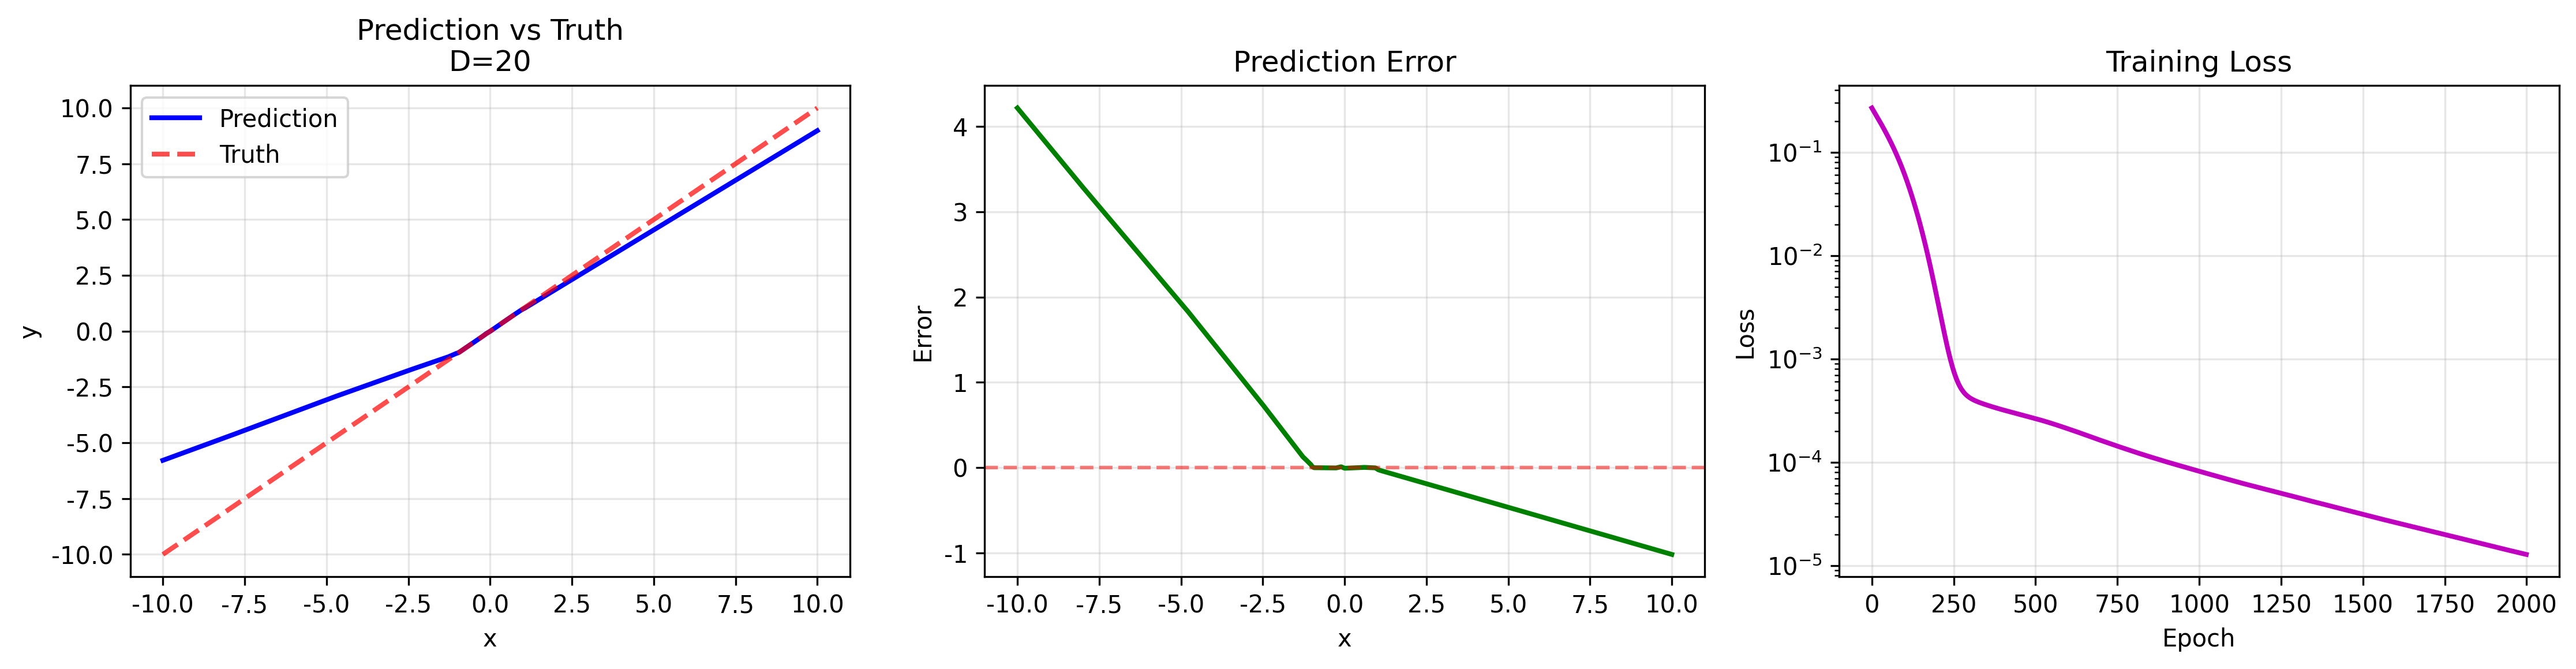
\includegraphics[width=\linewidth]{linear D20.png}
    \caption{linear D20}
    \label{linear D20}
\end{figure}
\begin{figure}[htbp]
    \centering
    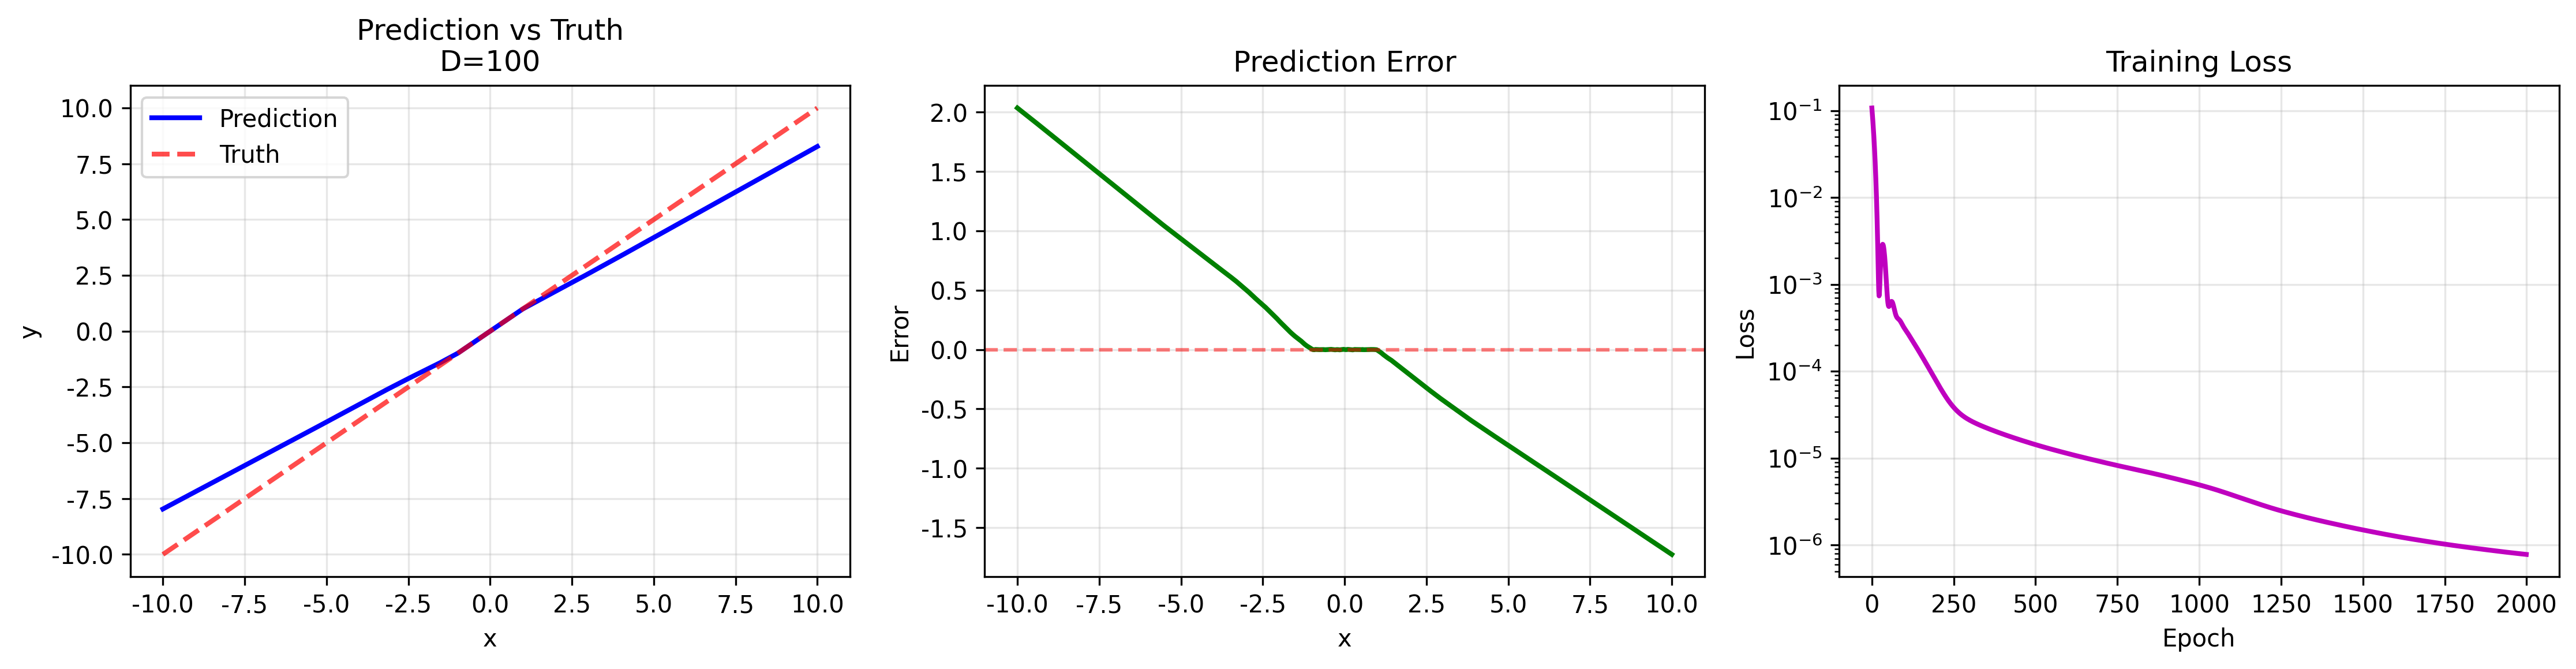
\includegraphics[width=\linewidth]{linear D100.png}
    \caption{linear D100}
    \label{linear D100}
\end{figure}
\begin{figure}[htbp]
    \centering
    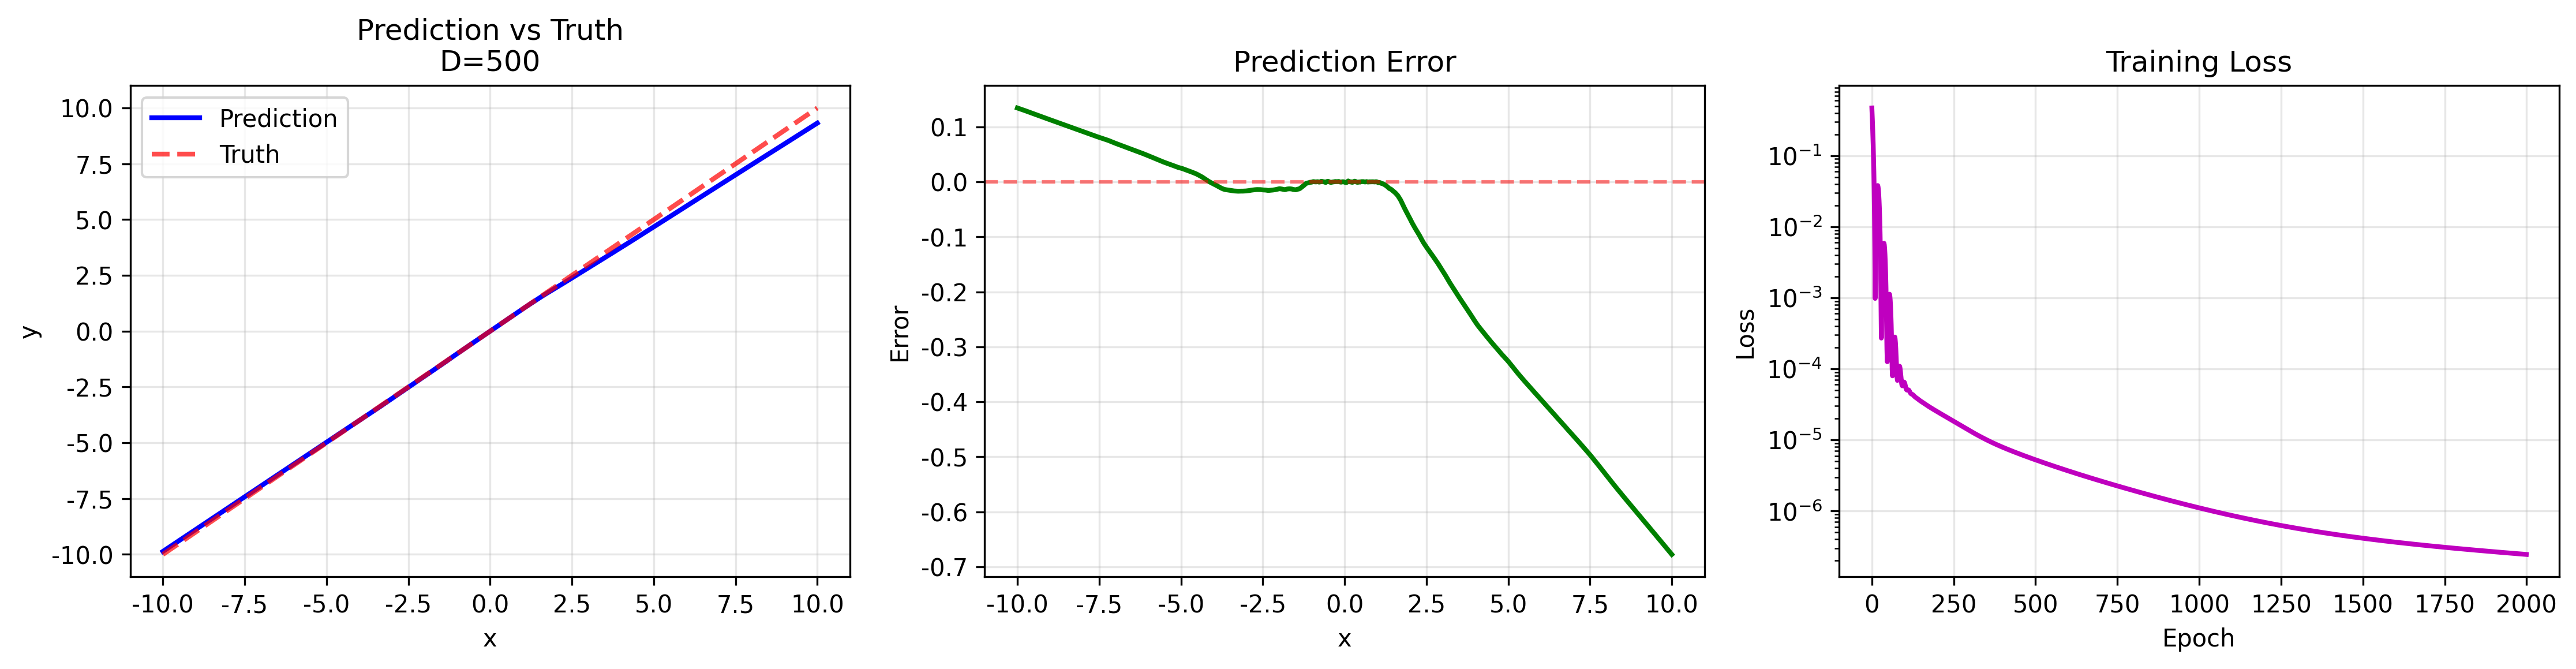
\includegraphics[width=\linewidth]{linear D500.png}
    \caption{linear D500}
    \label{linear D500}
\end{figure}
从理论分析和数值结果中可以得到：
\begin{itemize}
    \item 线性函数$y=x$可以被两层神经网络精确表示，原因是两层ReLU可以表示连续分段线性函数。具体而言，$f(x)=x=\text{ReLU}(x)-\text{ReLU}(-x)$。
    以$D=2$为例，取$W^{(1)}=[1,1]^T,b^{(1)}=[0,0]^T,W^{(2)}=[1,-1],b^{(2)}=0$即可。
    而对$D>2$是类似的，只需要取多余分量均为0即可。
    \item 从数值结果看，通过该神经网络学到的是分段线性函数，在测试数据范围内，随着D增大，内插误差逐渐减小到1e-2内，
    外推误差也呈现减小趋势，最终误差较小，基本可以认为信任此预测，表明逐渐逼近线性函数。
    但是得到的结果始终不是全局线性函数，而是分段线性函数，所以神经网络的训练没有找到这样的精确表示，但是找到了较为近似的表示。
\end{itemize}

\subsection{二次函数}
\subsubsection{参数设置}
学习率lr=0.0001，epoch=5000，D=[2, 10, 50, 100, 500, 1000]。
\subsubsection{数值结果}
首先用表格展示。
\begin{table}
    \centering
    \begin{tabular}{c c c c c}
        \hline
        D&内插最大误差&内插平均误差&外推最大误差&外推平均误差\\
        2&0.66&0.26&100&36.8\\
        10&0.40&0.11&98.1&34.0\\
        50&8e-2&1.6e-2&91.6&30.8\\
        100&4.3e-2&5.0e-3&85.8&29.4\\
        500&3.7e-3&9.7e-4&85.4&28.7\\
        1000&1.8e-3&3.6e-4&85.1&28.7\\
    \end{tabular}
    \caption{二次函数}
    \label{二次函数}
\end{table}
下面用图片展示数值结果，包括真实函数与预测函数曲线对比、预测误差曲线、训练Loss下降曲线。
\begin{figure}[htbp]
    \centering
    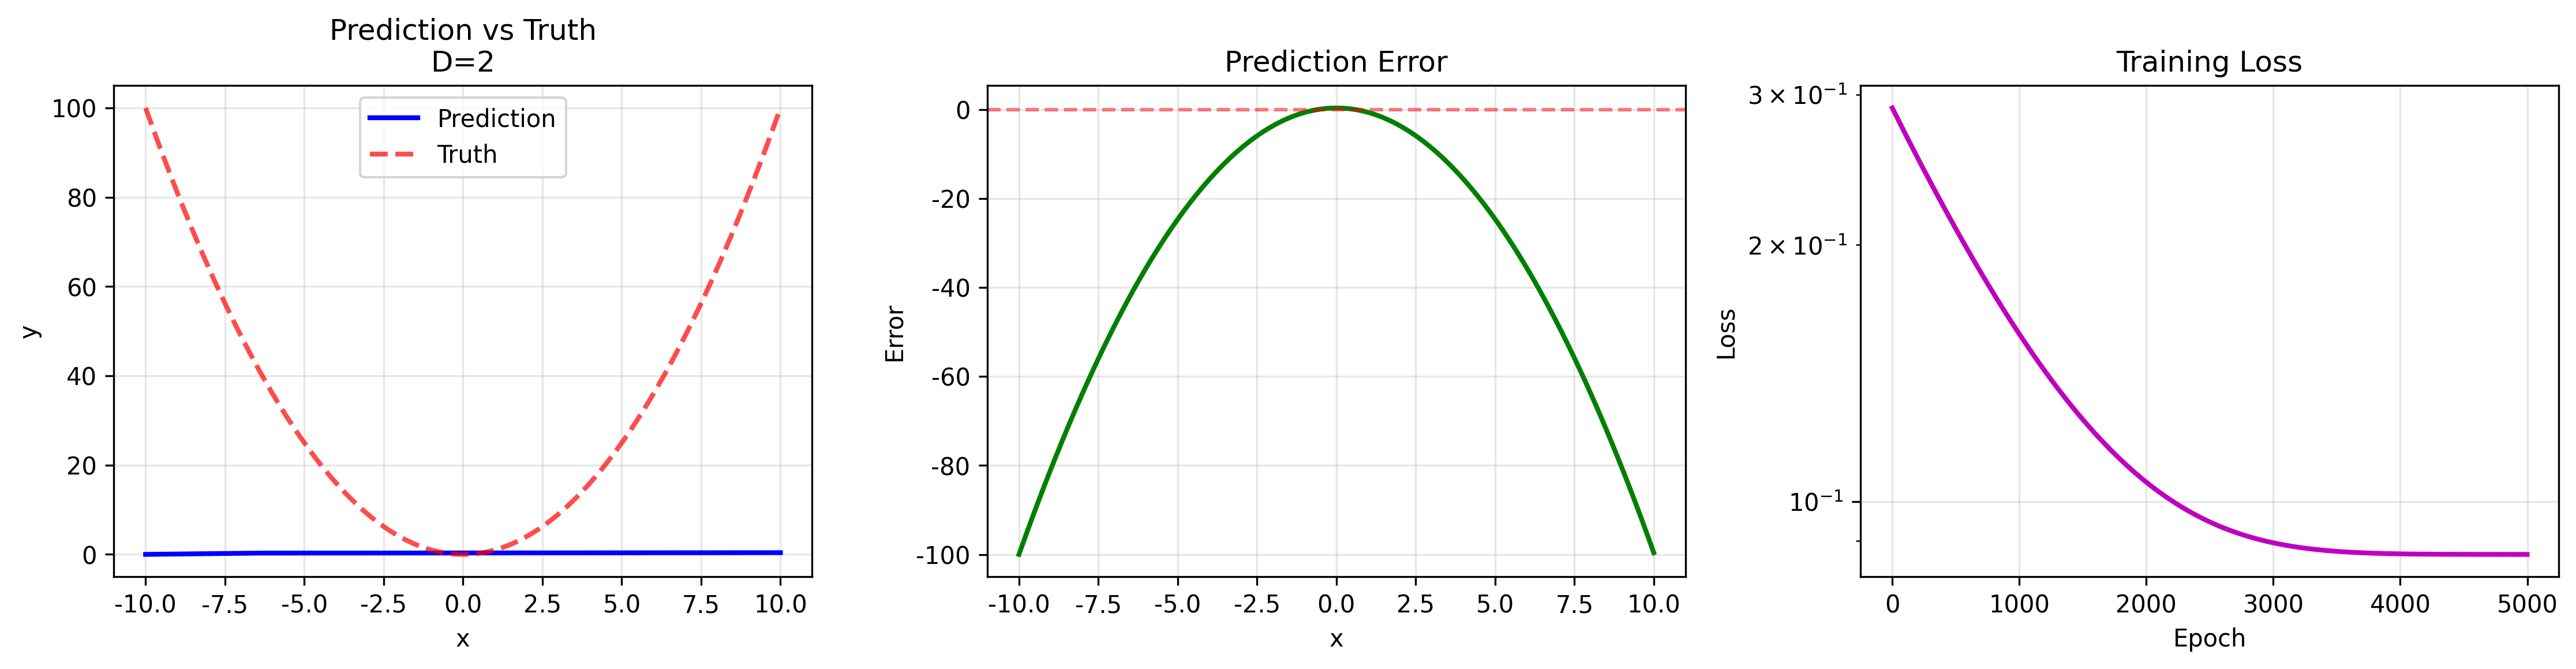
\includegraphics[width=\linewidth]{quadratic D2.png}
    \caption{quadratic D2}
    \label{quadratic D2}
\end{figure}
\begin{figure}[htbp]
    \centering
    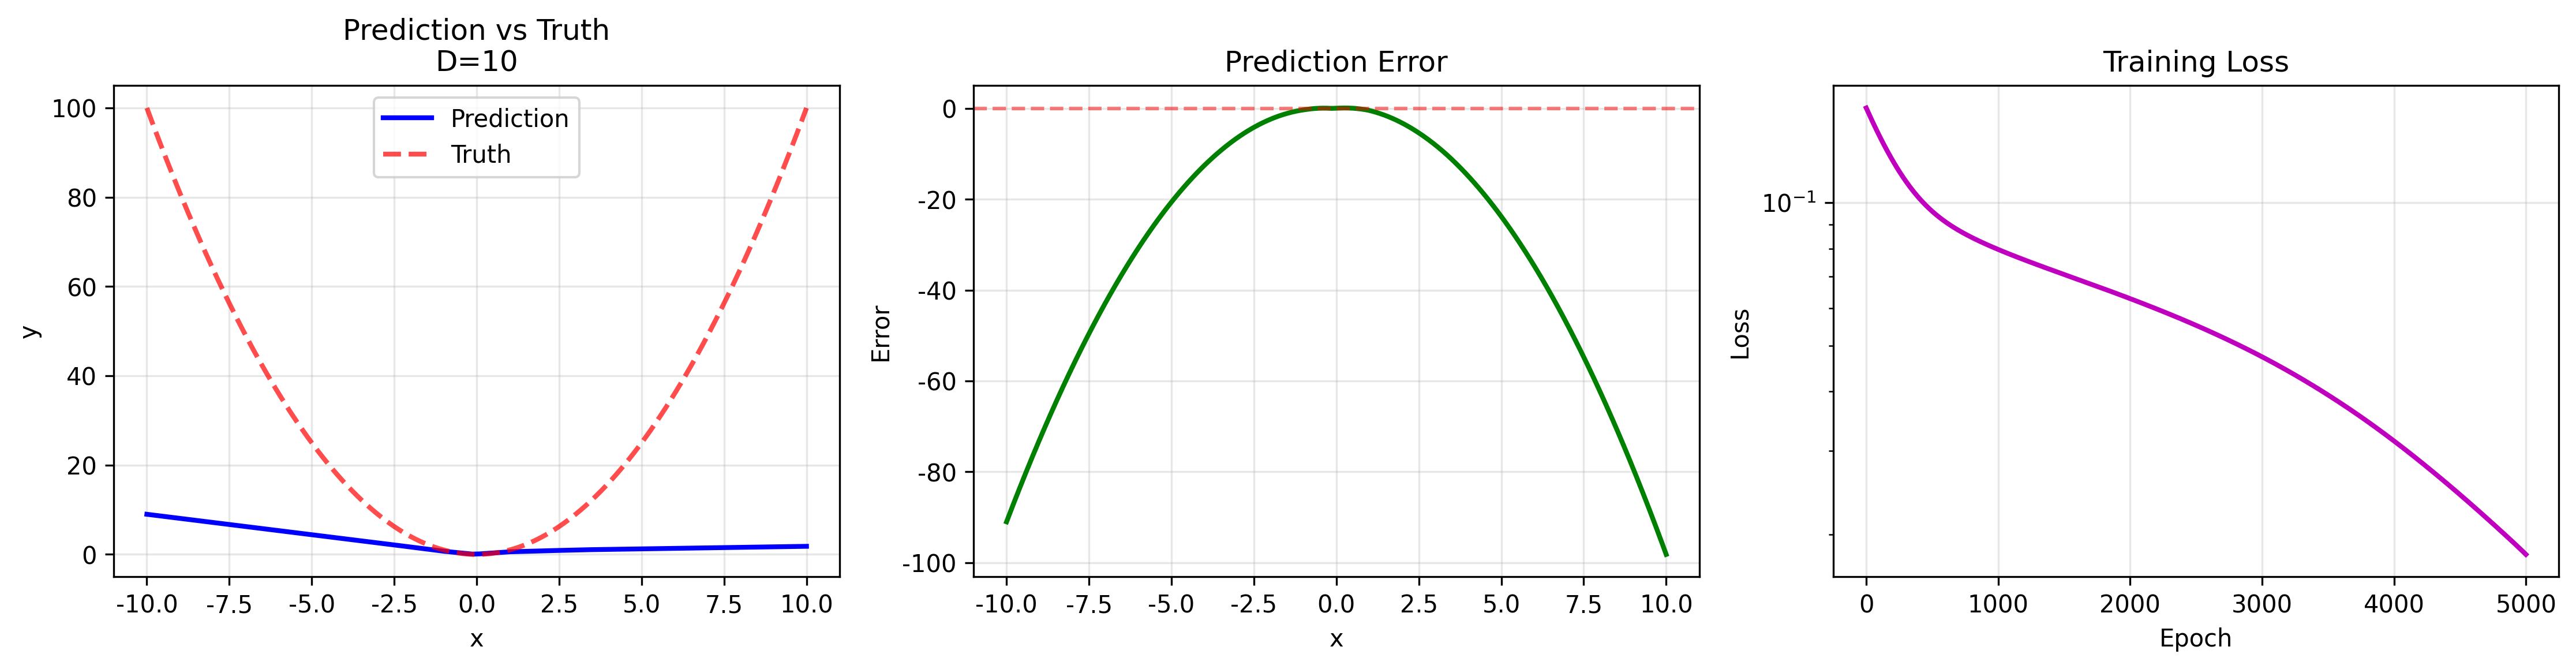
\includegraphics[width=\linewidth]{quadratic D10.png}
    \caption{quadratic D10}
    \label{quadratic D10}
\end{figure}
\begin{figure}[htbp]
    \centering
    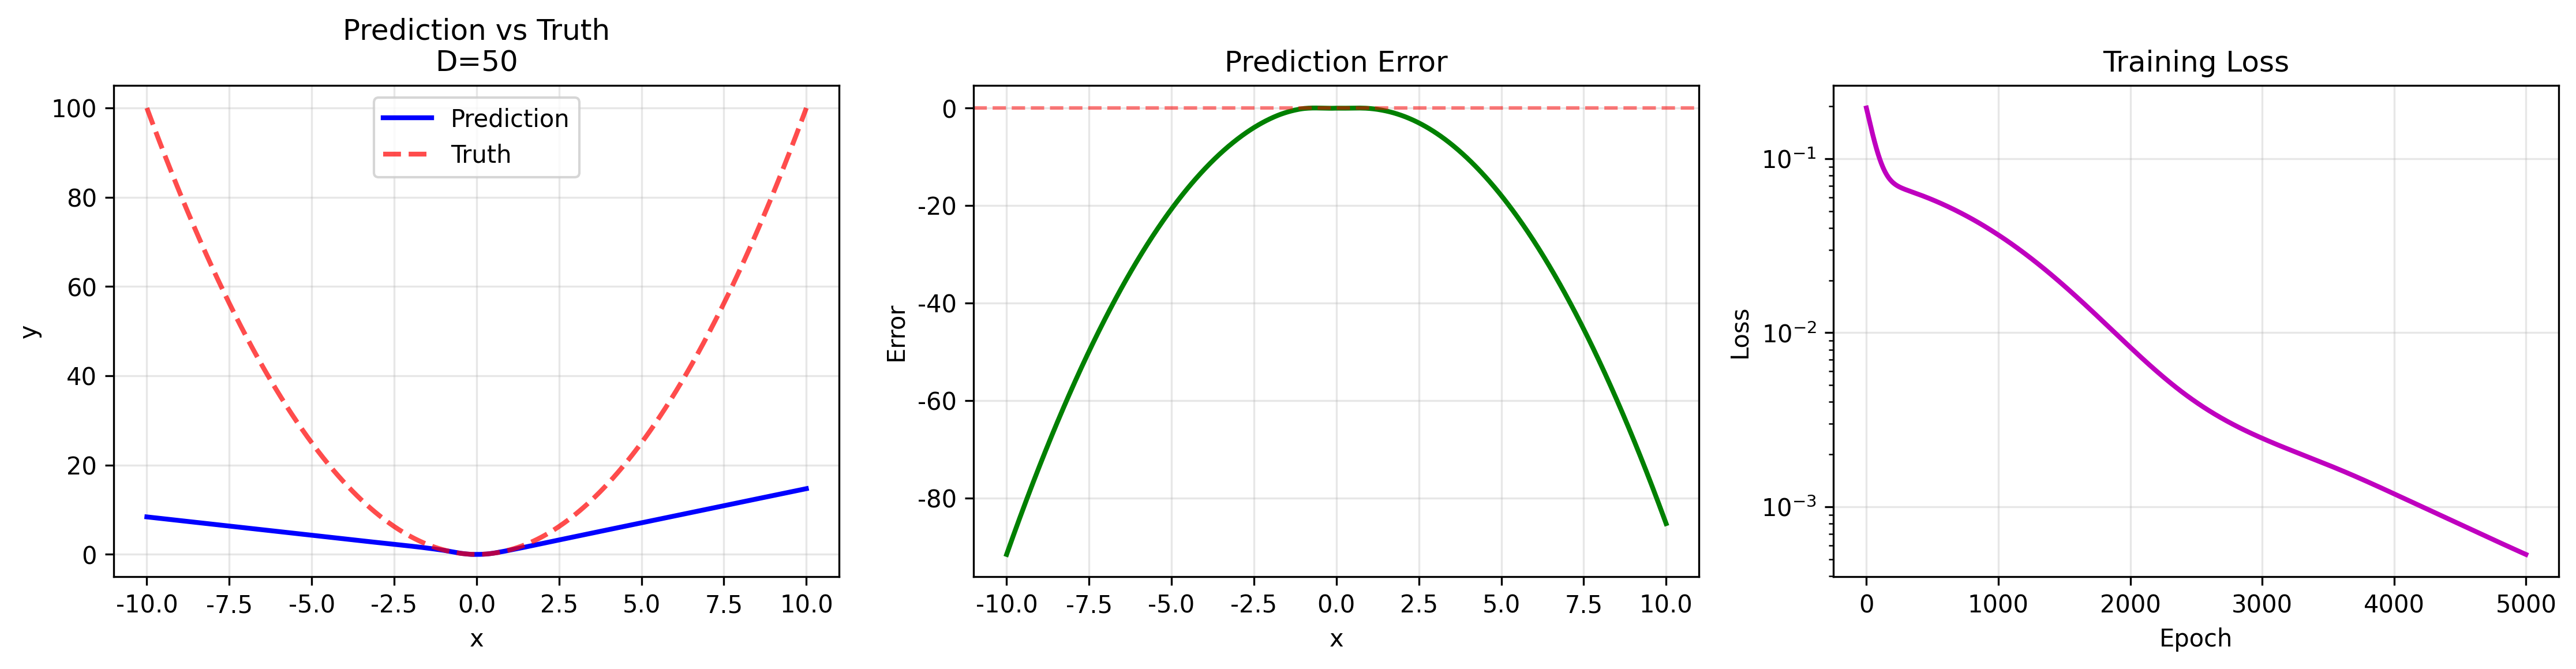
\includegraphics[width=\linewidth]{quadratic D50.png}
    \caption{quadratic D50}
    \label{quadratic D50}
\end{figure}
\begin{figure}[htbp]
    \centering
    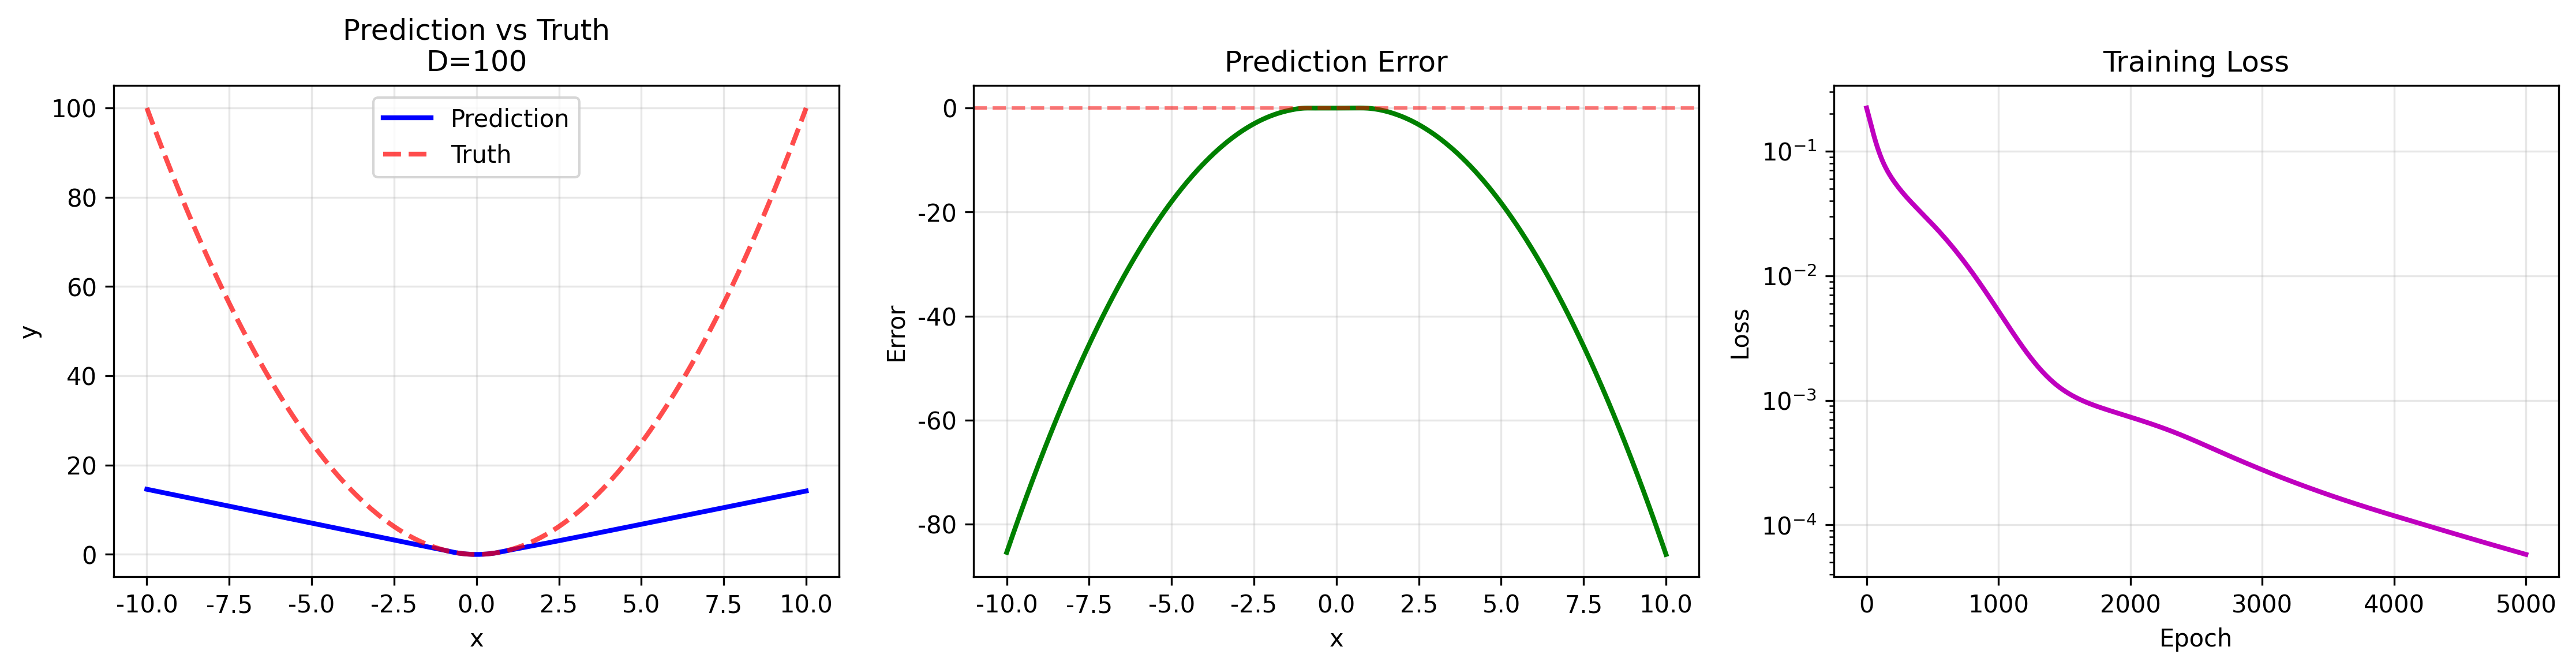
\includegraphics[width=\linewidth]{quadratic D100.png}
    \caption{quadratic D100}
    \label{quadratic D100}
\end{figure}
\begin{figure}[htbp]
    \centering
    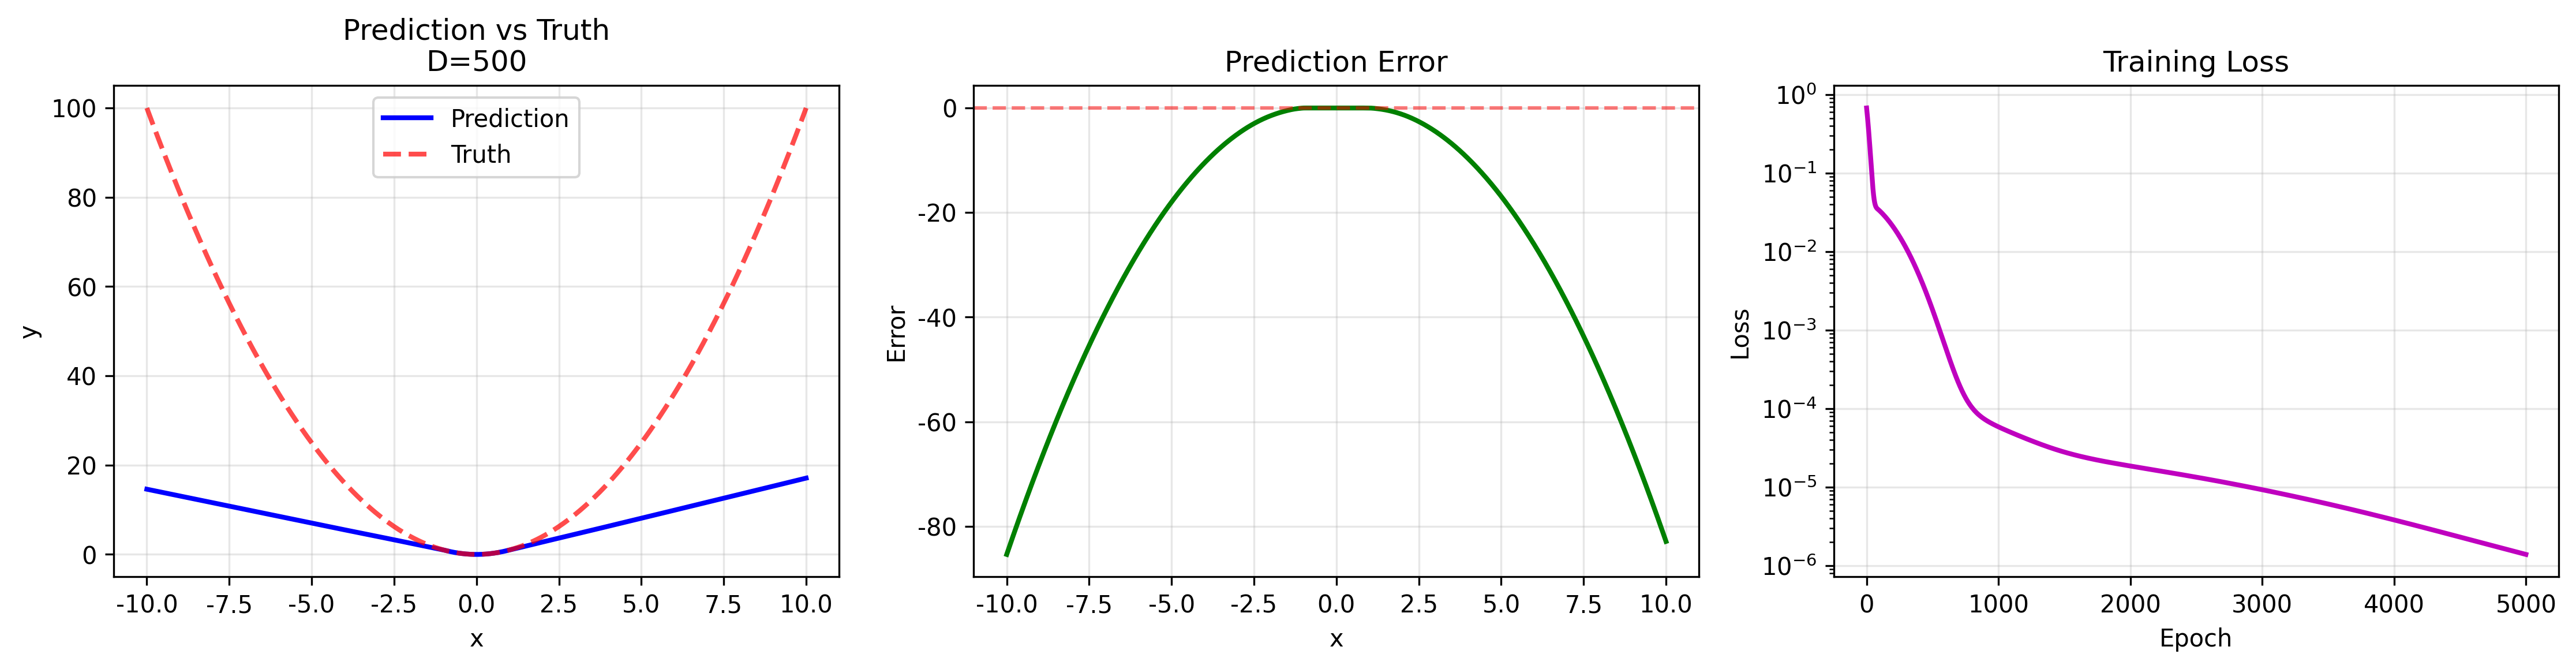
\includegraphics[width=\linewidth]{quadratic D500.png}
    \caption{quadratic D500}
    \label{quadratic D500}
\end{figure}
\begin{figure}[htbp]
    \centering
    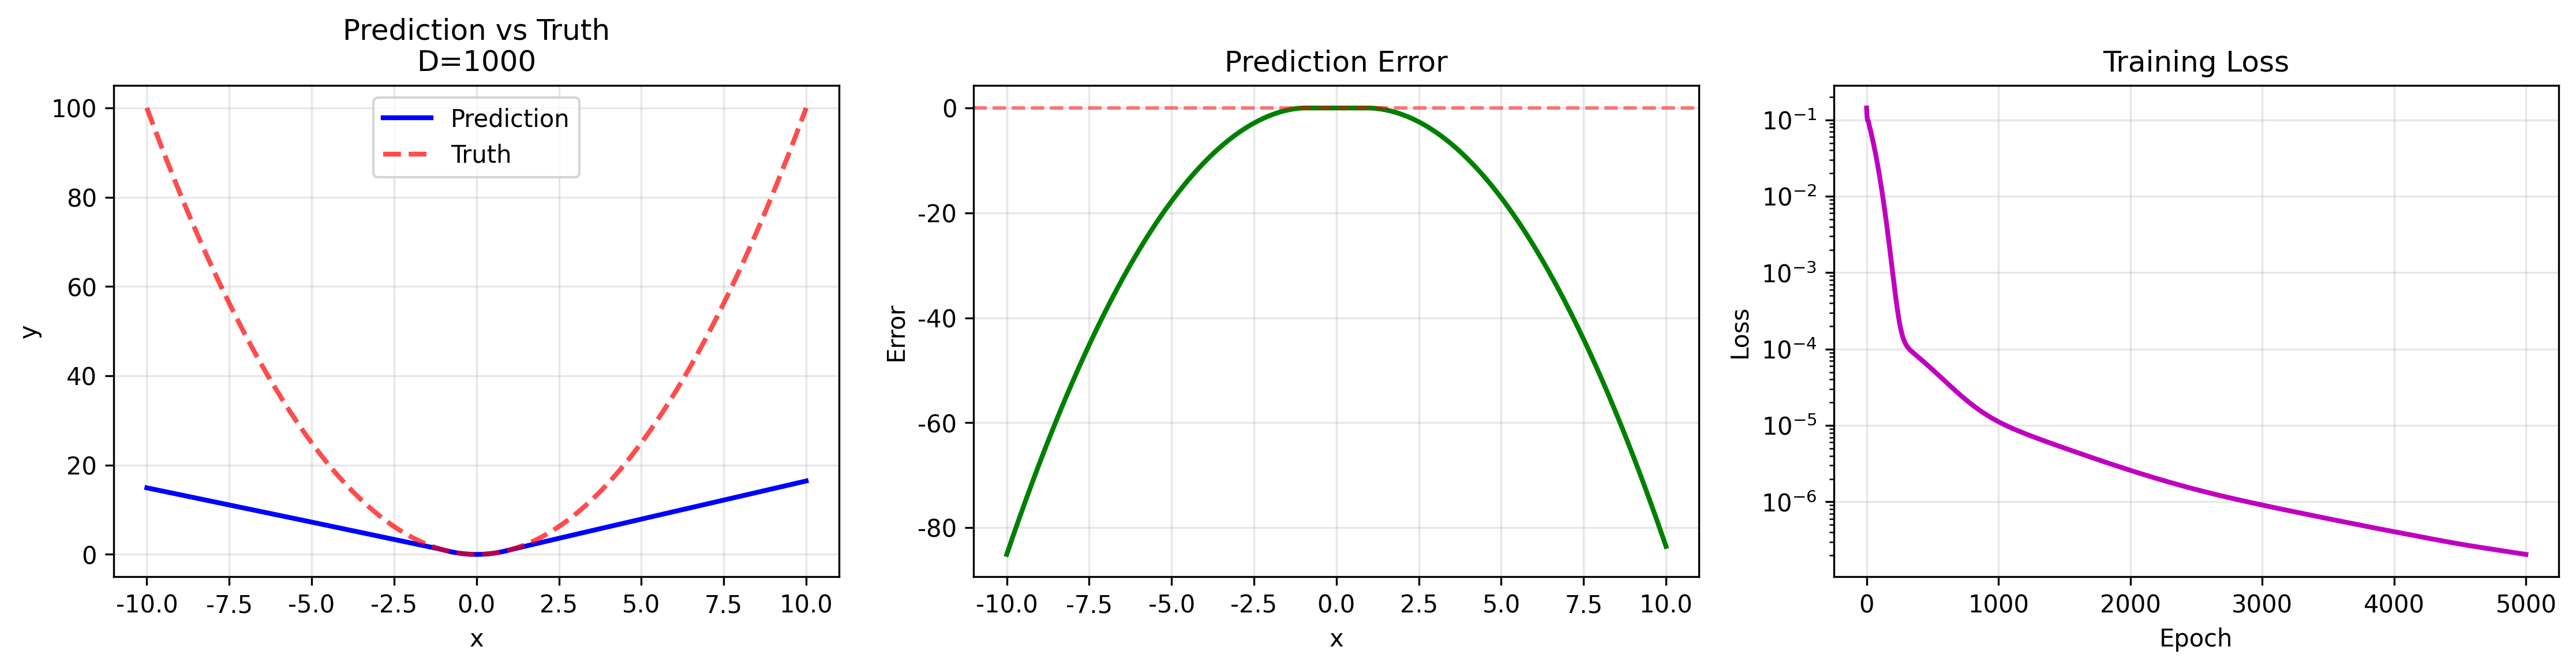
\includegraphics[width=\linewidth]{quadratic D1000.png}
    \caption{quadratic D1000}
    \label{quadratic D1000}
\end{figure}
从理论分析和数值结果中可以得到：
\begin{itemize}
    \item 二次函数$y=x^2$不可以被两层神经网络精确表示，原因是两层ReLU可以表示连续分段线性函数，但无法表达二次函数。
    \item 从数值结果看，通过该神经网络学到的是分段线性函数，在测试数据范围内，随着D增大，内插误差减小到1e-2内，
    但外推误差虽然在减小，但数值很大，维持在85以上，无法信任此预测，这表明该预测并未全局拟合二次函数。
    \item 原因分析：在$[-1,1]$内，神经网络训练得到的是分段线性函数，其斜率大致在1.0-2.0之间。合理假设所预测的斜率是1.5左右，
    则代入可得在$x=10,-10$的预测值为15，所以误差大约为85。
    \item 改进方法：重新选择更合适的激活函数和网络架构，比如增加神经网络深度。
\end{itemize}


\subsection{正弦函数}
\subsubsection{参数设置}
学习率lr=0.00001，epoch=10000，D=[2, 10, 50, 100, 500, 1000]。
\subsubsection{数值结果}
首先用表格展示。
\begin{table}
    \centering
    \begin{tabular}{c c c c c}
        \hline
        D&内插最大误差&内插平均误差&外推最大误差&外推平均误差\\
        2&1.04&0.64&1.31&0.65\\
        10&1.05&0.65&1.8&0.70\\
        50&1.09&0.64&6.28&1.96\\
        100&1.09&0.64&5.71&2.11\\
        500&1.18&0.62&16.2&7.37\\
        1000&1.12&0.61&27.0&12.2\\
    \end{tabular}
    \caption{正弦函数}
    \label{正弦函数}
\end{table}
下面用图片展示数值结果，包括真实函数与预测函数曲线对比、预测误差曲线、训练Loss下降曲线。
\begin{figure}[htbp]
    \centering
    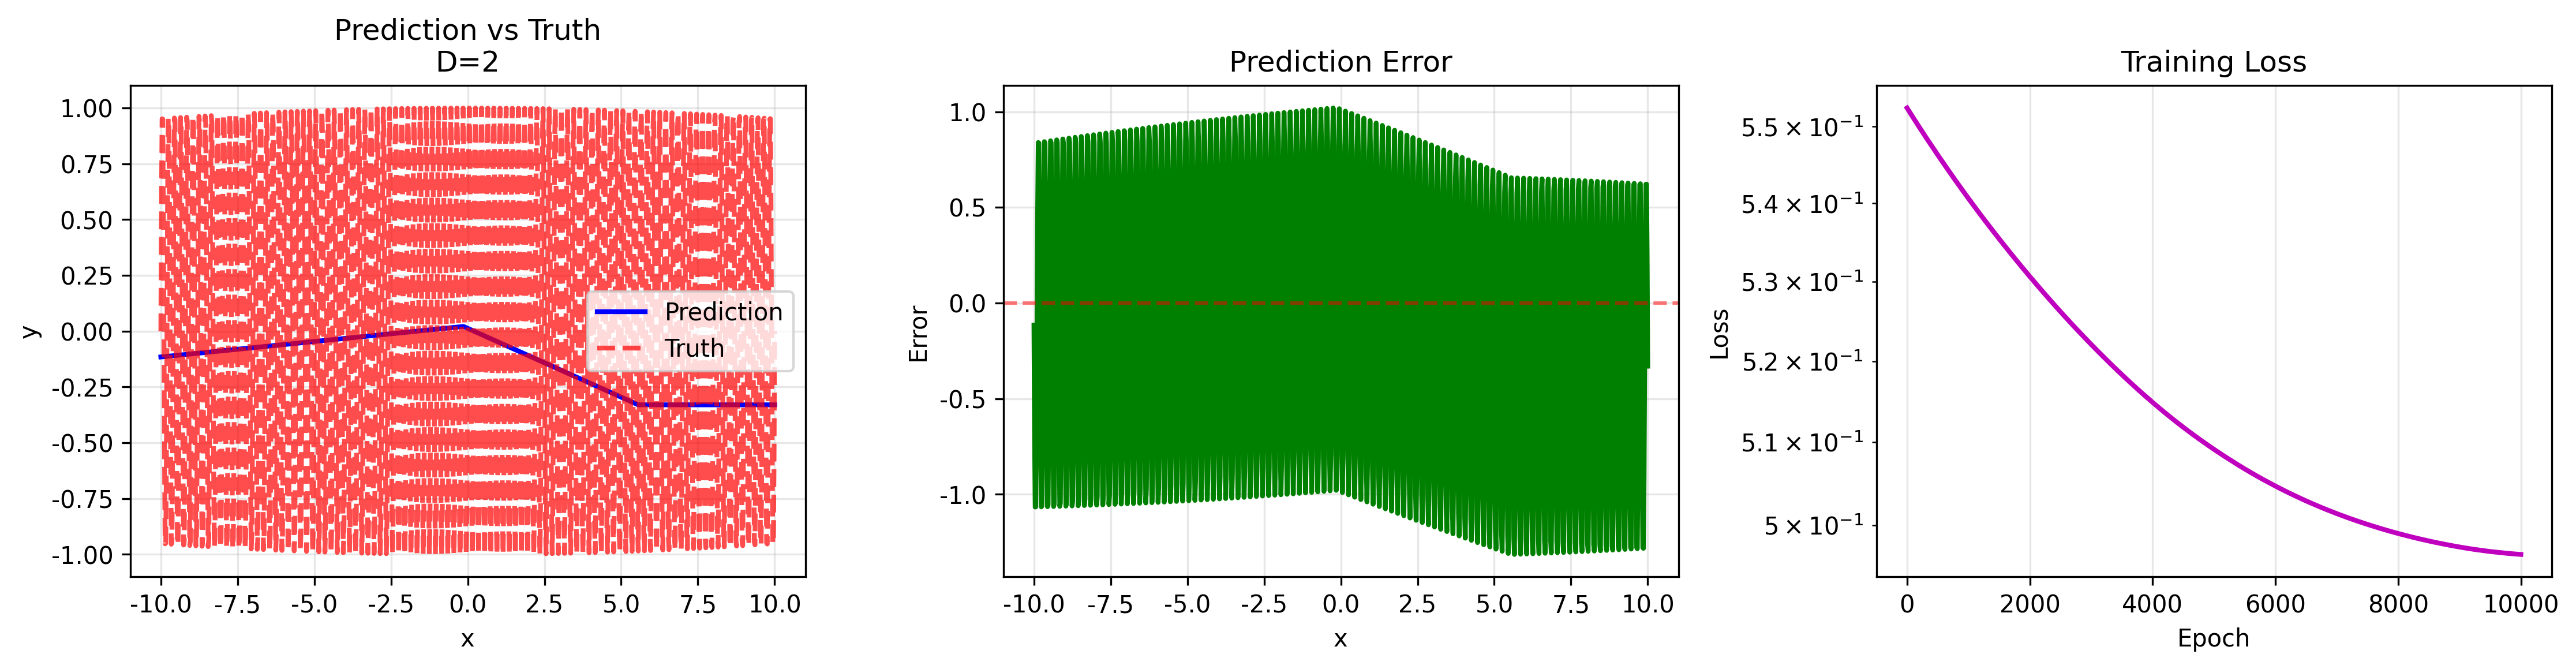
\includegraphics[width=\linewidth]{sine D2.png}
    \caption{sine D2}
    \label{sine D2}
\end{figure}
\begin{figure}[htbp]
    \centering
    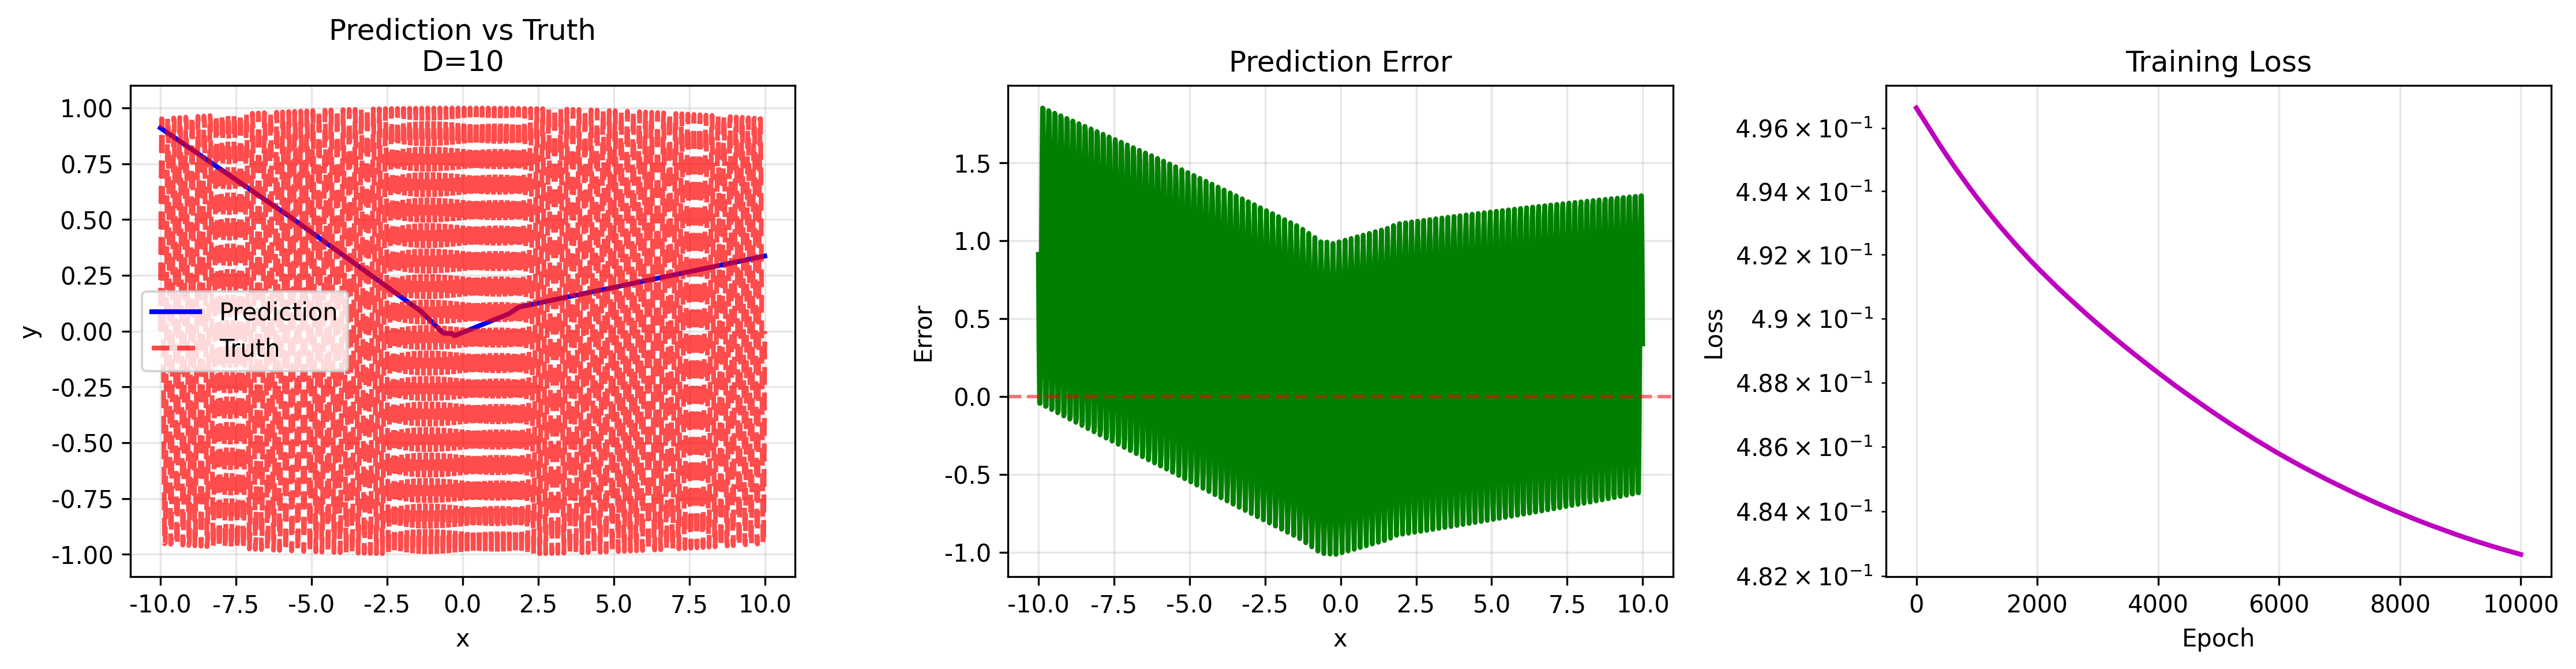
\includegraphics[width=\linewidth]{sine D10.png}
    \caption{sine D10}
    \label{sine D10}
\end{figure}
\begin{figure}[htbp]
    \centering
    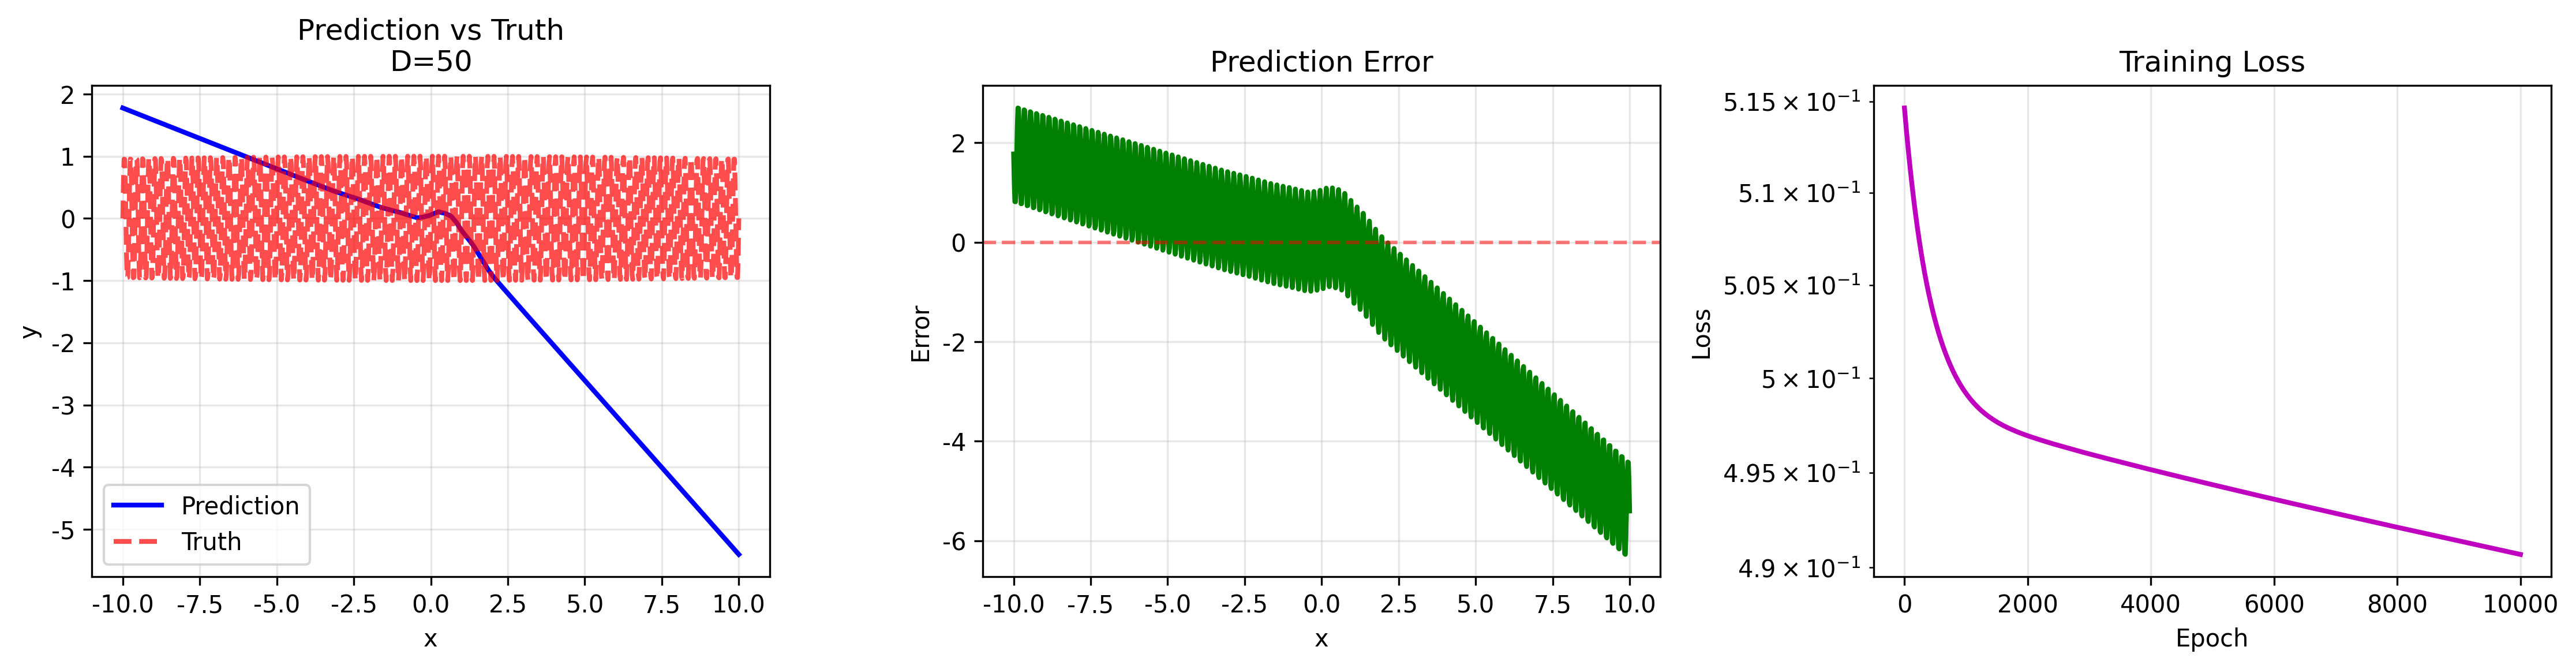
\includegraphics[width=\linewidth]{sine D50.png}
    \caption{sine D50}
    \label{sine D50}
\end{figure}
\begin{figure}[htbp]
    \centering
    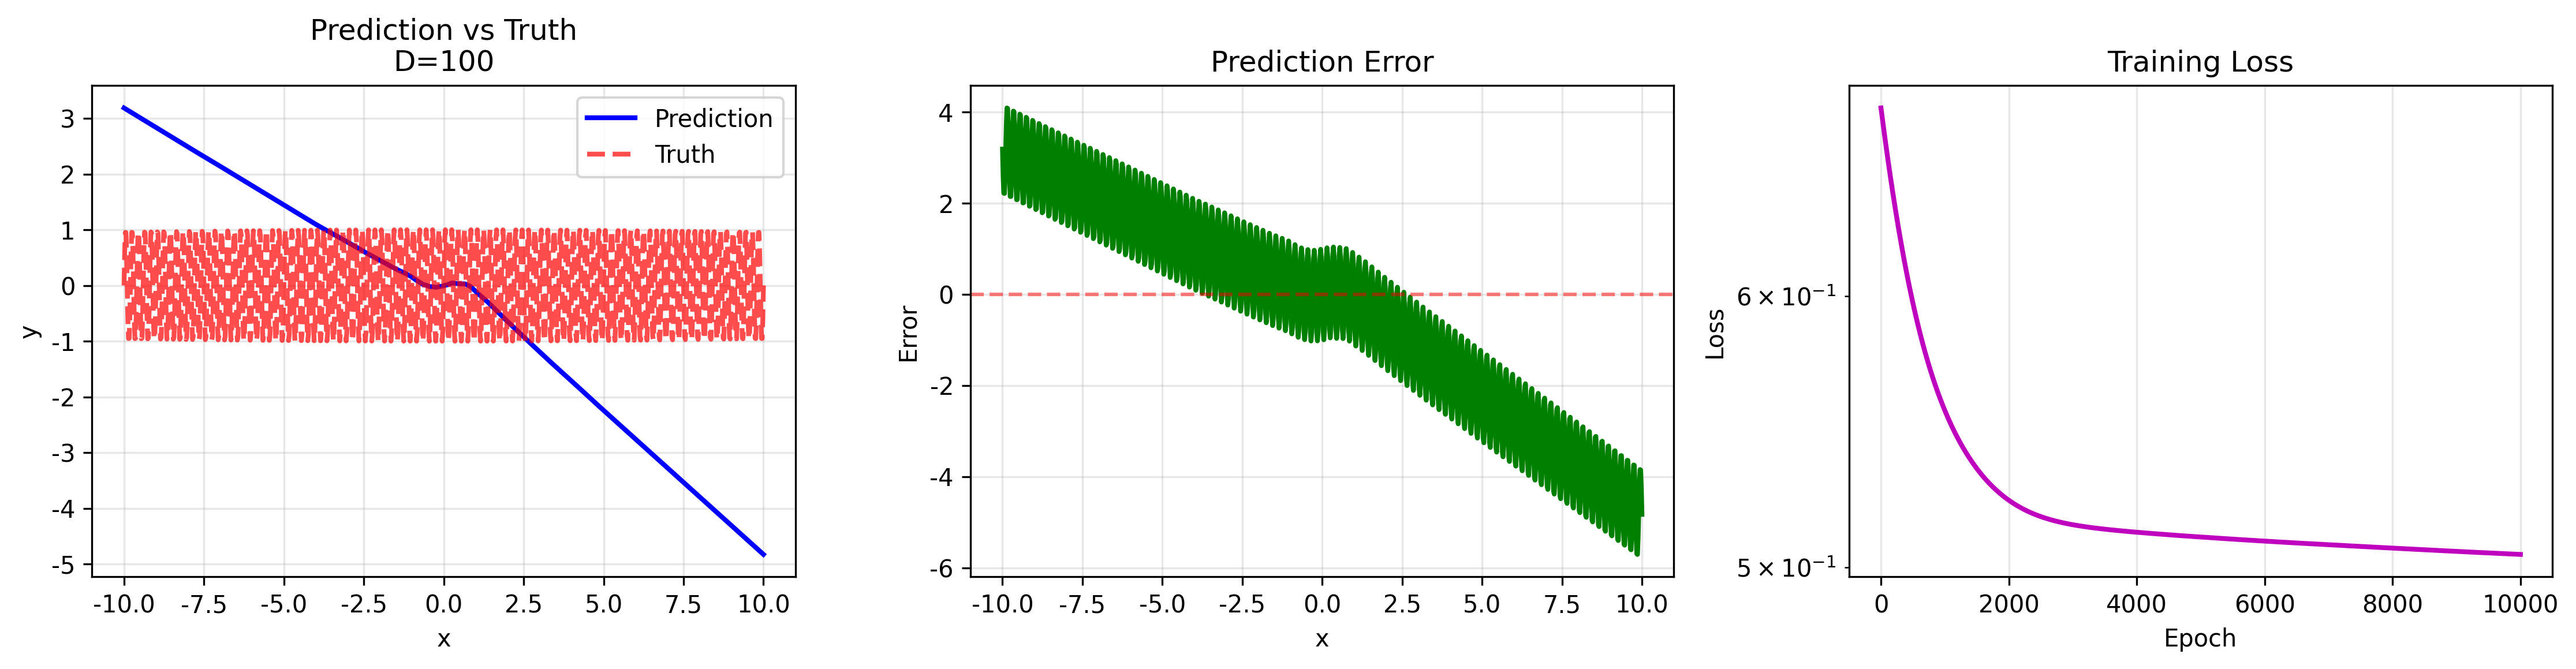
\includegraphics[width=\linewidth]{sine D100.png}
    \caption{sine D100}
    \label{sine D100}
\end{figure}
\begin{figure}[htbp]
    \centering
    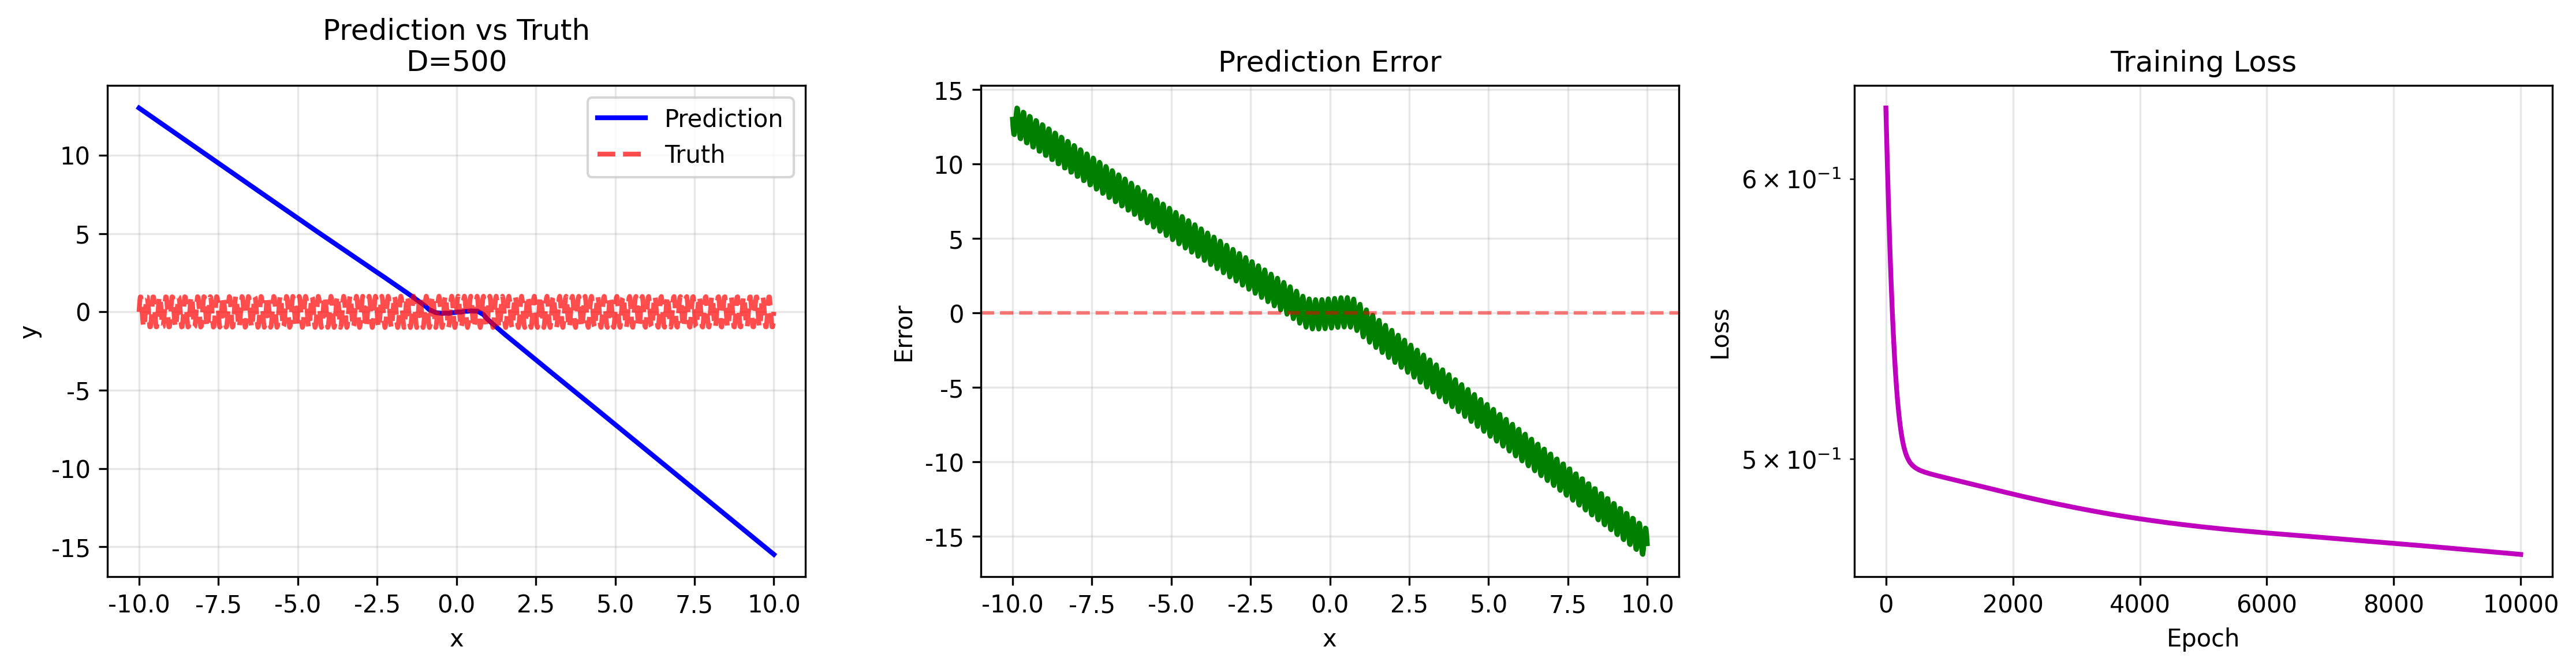
\includegraphics[width=\linewidth]{sine D500.png}
    \caption{sine D500}
    \label{sine D500}
\end{figure}
\begin{figure}[htbp]
    \centering
    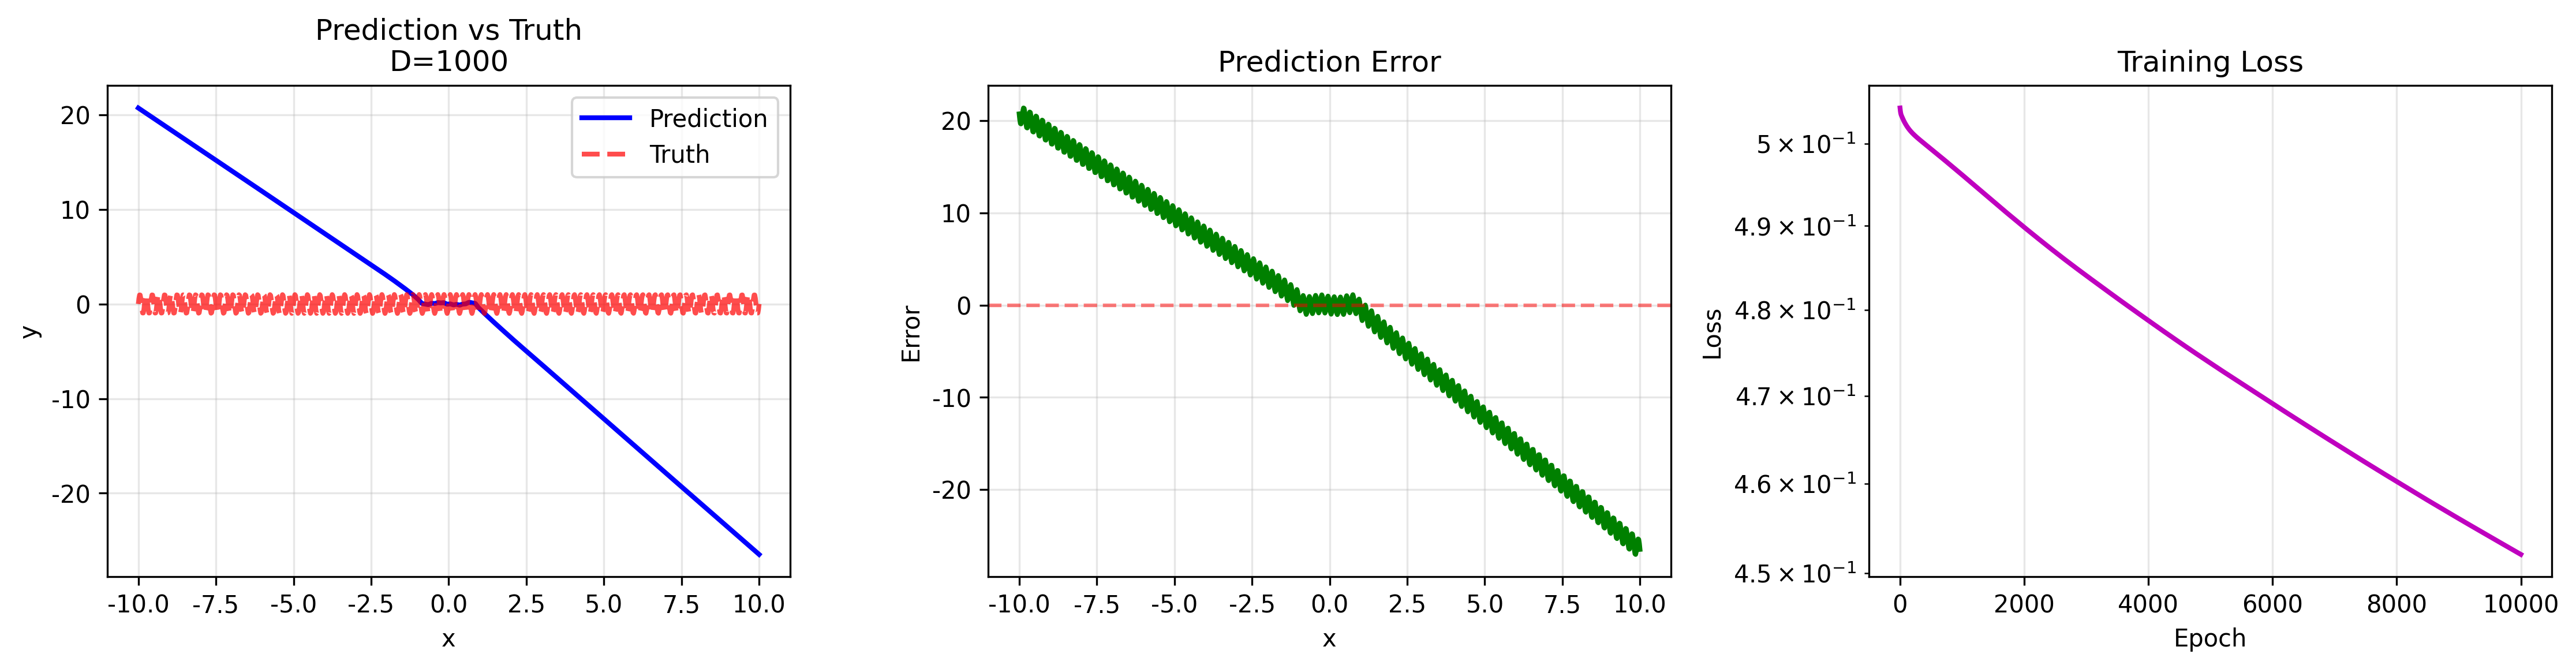
\includegraphics[width=\linewidth]{sine D1000.png}
    \caption{sine D1000}
    \label{sine D1000}
\end{figure}
从理论分析和数值结果中可以得到：
\begin{itemize}
    \item 正弦函数$y=\sin (10\pi x)$不可以被两层神经网络精确表示，原因是两层ReLU可以表示连续分段线性函数，但无法表达正弦函数。
    \item 从数值结果看，通过该神经网络学到的是分段线性函数，在测试数据范围内，随着D增大，内插误差基本不变，
    外推误差呈现增大的趋势，无法信任此预测。
    \item 原因分析：在$[-1,1]$内，神经网络训练得到的是分段线性函数。由于原函数高度振荡，分段线性函数完全无法捕捉此特征行为。
    \item 改进方法：重新选择更合适的激活函数和网络架构，比如增加神经网络深度。
\end{itemize}

\section{卷积神经网络}
\subsection{问题描述}
学习使用手写数字图像数据集MNIST，考虑卷积神经网络进行手写数字图形的分类，详细描述搭建的网络，报告结果。
\subsection{数值方法}
使用pytorch搭建卷积神经网络，损失函数使用交叉熵CrossEntropyLoss，优化器为Adam。
\subsection{网络描述}
输入层：输入维度$1\times 28 \times 28\rightarrow$ \\
第一卷积层：提取32种特征，卷积核$3\times 3$，激活函数ReLU，输出维度$32\times 28 \times 28\rightarrow$\\
第一池化层：最大化$2\times 2$区域，输出维度$32\times 14 \times 14\rightarrow$\\
第二卷积层：提取64种特征，卷积核$3\times 3$，激活函数ReLU，输出维度$64\times 14 \times 14\rightarrow$\\
第二池化层：最大化$2\times 2$区域，输出维度$64\times 7 \times 7\rightarrow$\\
展平操作：输出维度$64\times 7 \times 7=3136\rightarrow$\\
第一Dropout层：丢弃率0.25，$\rightarrow$\\
第一全连接层：激活函数ReLU，输入输出维度$3136\rightarrow 128\rightarrow$\\
第二Dropout层：丢弃率0.50，$\rightarrow$\\
输出层：第二全连接层，无激活函数，输入输出维度$128\rightarrow 10$。
\subsection{参数设置}
学习率lr=0.001，Epoch=10。
\subsection{数值结果}
当Epoch=10，最终结果：Loss=0.0351，Accuracy=98.90\%，Test Accuracy=99.31\%。训练曲线如图\ref{cnn results}所示，包括Loss下降曲线和Accuracy上升曲线。
\begin{figure}[htbp]
    \centering
    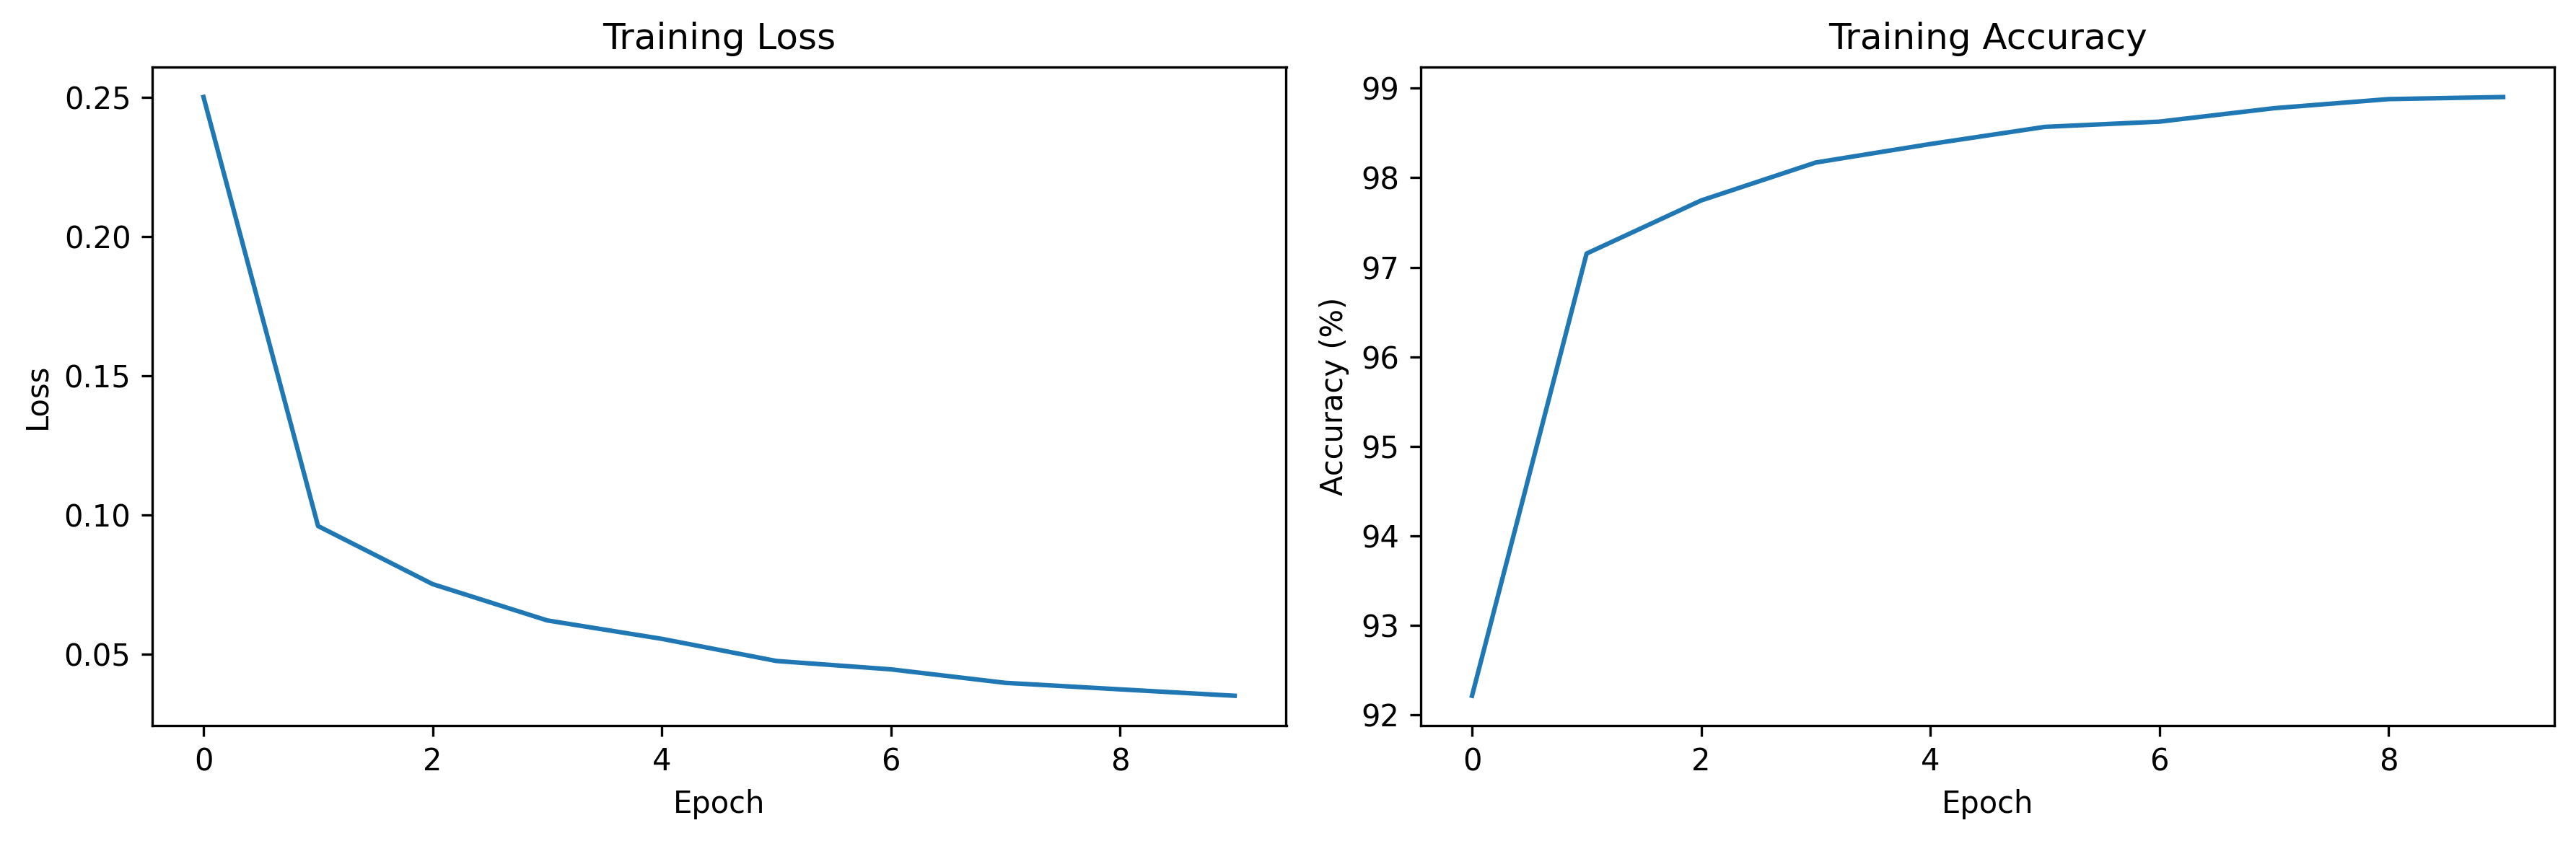
\includegraphics[width=\linewidth]{cnn results.png}
    \caption{cnn results}
    \label{cnn results}
\end{figure}
\end{document}